\documentclass[11pt, a4paper]{report}

% --- Packages ---
\usepackage[utf8]{inputenc}
\usepackage[T1]{fontenc}
\usepackage{lmodern}
\usepackage{geometry}
\geometry{a4paper, margin=1in}
\usepackage{amsmath, amssymb, amsfonts}
\usepackage{booktabs}
\usepackage{float}
\usepackage{graphicx}
\usepackage{hyperref}
\usepackage{caption}
\usepackage{array}
\usepackage{titlesec}
\usepackage{tabularx}
\usepackage{ragged2e}
\usepackage[table]{xcolor}
\usepackage{parskip}

% --- Document Info ---
\titleformat{\chapter}[hang]{\huge\bfseries}{\thechapter.\ }{0pt}{\huge\bfseries}
\titlespacing*{\chapter}{0pt}{-20pt}{20pt}
\title{State Space Models for Event-Based Object Detection: A Controlled Architectural Study with a Neuromorphic Deployment Path}
\author{Benas Vaiciulis}
\date{November 2026}

% --- added for the final thesis ---

% \tbd{...} marks prose still to be written. Set \tbdshowfalse before submission to hide
% every marker in one place (they will then render as nothing, and the document is clean).
% (xcolor is already loaded with the [table] option in the preamble above.)
\newif\iftbdshow \tbdshowtrue
\newcommand{\tbd}[1]{\iftbdshow{\color{red}\small\textbf{[TO WRITE: }\textit{#1}\textbf{]}}\fi}
\newcommand{\needsgpu}[1]{\iftbdshow{\color{orange!80!black}\small\textbf{[PENDING RUN: }\textit{#1}\textbf{]}}\fi}

\begin{document}

% --- Title Page ---
\begin{titlepage}
    \centering
    \vspace*{1cm}
    \Large\textbf{State Space Models for Event-Based Object Detection:}\\[4pt]
    \Large\textbf{A Controlled Architectural Study with a Neuromorphic Deployment Path} \\
    \vspace{0.5cm}
    \large Undergraduate Thesis --- MMAN4953 (Thesis C) \\
    \vspace{1.5cm}
    \textbf{Author:} Benas Vaiciulis \\
    \textbf{Supervisor:} Will Midgley\\
    \vspace{1.5cm}
    UNSW Sydney \\
    School of Mechanical and Manufacturing Engineering \\
    \vfill
    November 2026
\end{titlepage}

% --- Abstract ---
\begin{abstract}
Event cameras report per-pixel brightness changes asynchronously, with microsecond latency and very
high dynamic range --- properties well matched to perception under the size, weight and power (SWaP)
constraints of micro unmanned aerial vehicles. State space models (SSMs) have recently been proposed
as the natural sequence model for this data, but existing results confound several architectural
changes at once, leaving it unclear what an SSM actually contributes. This thesis isolates that
question. Starting from an exact reproduction of the S5-RVT baseline of Zubi\'c \emph{et al.}
(Gen1 test AP $=47.7$), two original detectors were built as \emph{controlled} backbone swaps into
the verified pipeline --- neck, detection head, loss, data pipeline and evaluator held fixed. The two
differ from each other only in the spatial mixer, so their comparison isolates that one architectural
change.

\textbf{EventSSM} (ResNet-18 convolutional spatial mixer with a Mamba-2 temporal recurrence) reaches
46.2 AP; \textbf{PureSSM} (bidirectional-Mamba spatial mixer, identical temporal path) reaches 46.4 AP
while being the smallest model (16.3\,M parameters), performing the least computation (10.0\,GFLOP,
best accuracy-per-FLOP at 4.63), and closing roughly half of the large-object gap to the attention
baseline ($\mathrm{AP}_L$ $+2.95$ over the convolutional hybrid). A gradient-based receptive-field
probe attributes that gain to a learned spatial extent up to twice that of the convolutional stack.
Under a true tenfold change in event rate PureSSM retains 69.7\% of its accuracy, the most of the
models tested\needsgpu{decision D1: add the same-protocol retention of RVT's ConvLSTM, measured on the
true-rate test set; the published 17.7\,\% used unreleased preprocessing}. An attempted
reproduction of the inference-time $\Delta t$-rescaling compensation reported in the literature finds
that, under the published checkpoint and code, it does not recover accuracy at any tested operating
point and the published high-rate result is not reproducible, while the rate robustness itself is
present without it.

\tbd{one to two sentences on the spiking SSM result once Stage 20--22 have run}

\end{abstract}

\tableofcontents

\chapter*{Nomenclature}
\addcontentsline{toc}{chapter}{Nomenclature}
\begin{tabular}{ll}
\multicolumn{2}{l}{\textit{Latin Symbols}} \\[4pt]
$A$ & state transition matrix \\
$\bar{A}$ & discretised state matrix \\
$B$ & input projection matrix \\
$\bar{B}$ & discretised input matrix \\
$C$ & contrast threshold \\
$C_{ssm}$ & SSM output projection matrix \\
$d_{model}$ & model embedding dimension \\
$h(t)$ & hidden state vector (continuous time) \\
$h(k)$ & latent state vector at discrete step $k$ \\
$L(x,y,t)$ & log luminance \\
$P$ & event polarity (+1 or -1) \\
$I$ & identity matrix \\
$t$ & time, s \\
$u(t)$ & input signal \\
$x, y$ & pixel coordinates \\[8pt]
\multicolumn{2}{l}{\textit{Greek Symbols}} \\[4pt]
$\Delta$, $\Delta t$ & SSM discretisation step size (used interchangeably) \\[8pt]
\multicolumn{2}{l}{\textit{Acronyms}} \\[4pt]
CNN & Convolutional Neural Network \\
DAVIS & Dynamic and Active-pixel Vision Sensor \\
DVS & Dynamic Vision Sensor \\
EST & Event Spike Tensor \\
GNN & Graph Neural Network \\
HDR & High Dynamic Range \\
LIF & Leaky Integrate-and-Fire \\
LTI & Linear Time-Invariant \\
RNN & Recurrent Neural Network \\
SNN & Spiking Neural Network \\
SSM & State Space Model \\
SSD & Single Shot MultiBox Detector \\
SWaP & Size, Weight, and Power \\
AP & Average Precision \\
BPTT & Backpropagation Through Time \\
ERF & Effective Receptive Field \\
FPN & Feature Pyramid Network \\
INRC & Intel Neuromorphic Research Community \\
IoU & Intersection over Union \\
mAP & mean Average Precision \\
NIR & Neuromorphic Intermediate Representation \\
PAFPN & Path Aggregation Feature Pyramid Network \\
SOP & Synaptic Operation \\
TBPTT & Truncated Backpropagation Through Time \\
UAV & Unmanned Aerial Vehicle \\
\end{tabular}

% --- Chapter 1: Introduction ---
\chapter{Introduction}
Micro unmanned aerial vehicles (UAVs) have emerged as transformative tools for applications ranging from infrastructure inspection and search-and-rescue operations to indoor mapping and environmental monitoring \cite{floreano2015science}; Australian regulation, for example, defines the micro class as remotely piloted aircraft of at most 250 grams \cite{casa2021part101}. Their small form factor enables navigation through confined spaces inaccessible to larger platforms; however, this advantage comes with severe constraints on payload capacity, onboard computational resources, and power budgets. These size, weight, and power (SWaP) limitations represent the central engineering challenge for autonomous micro-UAV systems: the perception and control pipeline must be both highly capable and extremely efficient.

Conventional frame-based cameras, while mature and well-supported by deep learning frameworks, suffer from inherent limitations that are particularly problematic for agile UAV flight. They capture redundant information at fixed frame rates, exhibit motion blur during rapid maneuvers, and possess limited dynamic range. 

Event-based cameras, also known as dynamic vision sensors (DVS), represent a paradigm shift in visual sensing. Unlike frame-based cameras, each pixel in an event camera independently and asynchronously responds to changes in log luminance, generating a stream of events with microsecond temporal resolution, a dynamic range exceeding 120 dB, and minimal motion blur \cite{gallego2020event}. These properties make event cameras inherently suited to the perception requirements of agile micro-UAVs, where rapid obstacle detection and avoidance are critical to safe operation. Several pioneering studies have demonstrated event-based obstacle avoidance on quadrotors \cite{falanga2020dynamic, sanket2020evdodgenet}, with perception latencies as low as 3.5 milliseconds \cite{falanga2020dynamic}. 

Despite these promising sensor characteristics, a significant gap remains in the algorithmic domain. Most existing approaches to processing event data for detection and avoidance rely on converting asynchronous event streams into frame-like representations for consumption by convolutional neural networks (CNNs) or recurrent neural networks (RNNs), thereby discarding much of the temporal richness that distinguishes event cameras from their frame-based counterparts. Transformer-based architectures, while capable of modelling long-range dependencies, have a computational cost quadratic in the number of tokens \cite{vaswani2017attention}, which weighs heavily on the severely resource-constrained processors typical of micro-UAVs. 

State Space Models (SSMs), and in particular the recently developed Mamba architecture and its variants, offer a compelling alternative. SSMs model input sequences through continuous-time linear dynamical systems that can be discretised at arbitrary time steps, achieving linear computational complexity while maintaining strong temporal reasoning capabilities \cite{gu2022efficiently}. Zubic et al. \cite{zubic2024state} have recently reported that SSMs accommodate the variable temporal resolution inherent to event camera data, degrading far less than RNN- or transformer-based approaches when deployed at inference frequencies other than the training frequency; Section~\ref{sec:robustness} re-examines that claim. 

This thesis investigates state space models for event-based object detection, motivated by the perception needs of micro-UAVs; obstacle avoidance is the motivating application rather than an evaluated system (Section~\ref{sec:scope}). The working hypothesis is that SSM-based backbones can exploit the temporal structure of event streams at least as well as convolutional, recurrent or transformer-based ones, with competitive accuracy and favourable efficiency. The research question below narrows this hypothesis to a form that can be tested. 

% --- Chapter 2: Literature Review ---


\section{Research Question}
\label{sec:rq}
Prior work establishes that state space models are \emph{competitive} on event-camera detection, but
every published comparison changes several things at once --- backbone, tokeniser and training recipe
together --- so the contribution of the sequence model itself cannot be read off the result. This
thesis narrows the question until it is answerable:

\begin{quote}
\textbf{Holding the entire detection pipeline fixed, what is the isolated effect of the backbone's
spatial mixer --- convolution versus state space --- on accuracy, temporal robustness and efficiency
for event-based object detection?}
\end{quote}

A second question follows from the first, and motivates the neuromorphic strand of the work:
\emph{what does it cost to make such a detector spiking, and what does neuromorphic hardware give back
in return?}

\section{Contributions}
\label{sec:contributions}
\begin{enumerate}
  \item An exact reproduction of the S5-RVT baseline (Gen1 test AP $47.7$), establishing a verified
        pipeline and evaluator against which all subsequent models are measured.
  \item \textbf{Two original detectors}, EventSSM and PureSSM, built as drop-in backbone swaps into
        that pipeline, giving a four-model ablation in which the own models differ from one another in
        one component each (the spatial mixer between EventSSM and PureSSM, the temporal readout between
        PureSSM and its spiking variant); against the published baseline, the whole backbone and two
        training settings differ.
  \item \textbf{A causal mechanism for the large-object result:} a gradient-based effective-receptive-field
        probe showing that the state-space spatial mixer sees up to twice as far as the convolutional
        stack, and --- unlike the convolutional stack --- \emph{widens its field through training}.
  \item \textbf{A reproduction study of $\Delta t$-rescaling:} under the published checkpoint and code,
        the inference-time compensation reported to give SSMs their temporal generalisation does not
        recover accuracy at any tested operating point (at a true tenfold rate it costs 9--13~mAP), and
        the published 200\,Hz result is not reproducible. The rate robustness itself is reproduced
        without the compensation.
  \item \textbf{An efficiency frontier reported honestly}, including the results that do not flatter
        the proposed model --- launch-bound wall-clock latency and a streaming state 31 times larger
        than the baseline's.
  \item \tbd{the spiking SSM contribution, stated once Stage 20--22 have run}
\end{enumerate}

\section{Scope}
\label{sec:scope}
The project as registered in Thesis~A included a fourth aim: integration of the detector with an
obstacle-avoidance controller in simulation, and physical micro-UAV testing if feasible. \textbf{That
aim was descoped}, and the effort redirected into the controlled architectural study and the
neuromorphic strand reported here. Section~\ref{sec:scope_change} states the justification in full.
The SWaP motivation for the work is unchanged; what changed is that the evaluation is architectural
rather than system-level.

\section{Thesis Organisation}
\label{sec:organisation}
Chapter~\ref{ch:lit} reviews event-based sensing, event representations, detection architectures,
state space models, spiking networks and neuromorphic hardware, and identifies the research gaps.
Chapter~\ref{ch:method} describes the frozen pipeline, the four models and the spiking block.
Chapter~\ref{ch:setup} gives the dataset, metrics, hardware and training protocol.
Chapter~\ref{ch:results} reports accuracy, mechanism, temporal robustness and efficiency.
Chapter~\ref{ch:discussion} interprets those results and states the limitations.
Chapter~\ref{ch:conclusion} concludes and sets out future work.

\chapter{Literature Review}
\label{ch:lit}

\section{Event-Based Cameras: Principles and Hardware}
Event-based cameras, or neuromorphic vision sensors, operate on a fundamentally different principle from conventional frame-based cameras. Rather than capturing synchronous frames at a fixed rate, each pixel independently monitors changes in log luminance and asynchronously emits an event when the change exceeds a predefined contrast threshold $C$. Formally, a pixel at coordinates $(x, y)$ generates an event $e = (x, y, t, p)$ at time $t$ when $|L(x, y, t) - L(x, y, t - \Delta t)| \geq C$, where $L$ denotes log luminance and $p \in \{+1, -1\}$ indicates the polarity of the brightness change \cite{gallego2020event}, \cite{lichtsteiner2008128x128}. This bio-inspired operating principle, modelled after biological retinal ganglion cells, confers several advantages over frame-based imaging: microsecond temporal resolution (typically 1 µs), very high dynamic range (>120 dB compared to approximately 60 dB for standard cameras), extremely low latency, low power consumption, and the absence of motion blur \cite{gallego2020event}.

Gallego et al. \cite{gallego2020event} provided a comprehensive survey of event-based vision, cataloguing the evolution of neuromorphic sensors from the original silicon retina proposed by Mahowald and Mead in 1992 through to modern commercially available sensors. The Dynamic Vision Sensor (DVS), developed at ETH Zurich, was among the first widely adopted event cameras and demonstrated the feasibility of asynchronous vision for robotics applications \cite{lichtsteiner2008128x128}. A significant advancement came with the Dynamic and Active-pixel Vision Sensor (DAVIS), which combines a DVS with a conventional active pixel sensor on the same die, enabling simultaneous capture of events and intensity frames at the same pixel locations \cite{brandli2014240x180}. The original DAVIS sensor, offering 240×180 pixel resolution, has become a widely used research platform, with later commercial variants such as the DAVIS346 extending this to higher resolutions. 

More recently, Prophesee (formerly Chronocam) has developed a series of commercial event cameras with increasing resolution and performance. The Gen3.1 sensors, used in the DSEC dataset \cite{gehrig2021dsec}, offer VGA-resolution event sensing, while the latest IMX636 sensor, developed in collaboration with Sony, provides 1280×720 HD resolution with ultra-high-speed operation \cite{prophesee2026metavision}. At the opposite end of the spectrum, the GenX320 sensor targets ultra-low-power applications with a 320×320 pixel array drawing about 3\,mW in typical operation and as little as 36\,$\mu$W in its lowest-power mode, making it particularly relevant for resource-constrained micro UAV platforms \cite{prophesee2025genx320}. The continued improvement in sensor resolution, noise characteristics, and power efficiency has been a key enabler for the expanding application of event cameras in robotics and autonomous systems. 

A notable limitation of current event cameras, however, is their relatively low spatial resolution compared to frame-based cameras. While modern frame-based sensors routinely achieve multi-megapixel resolutions, event cameras remain in the VGA to HD range. Furthermore, event cameras produce no output in static scenes, which can be both an advantage (data efficiency) and a limitation (loss of static scene information). These characteristics necessitate careful algorithm design that leverages the temporal strengths of event cameras while mitigating their spatial limitations.

\begin{figure}[htbp]
    \centering
    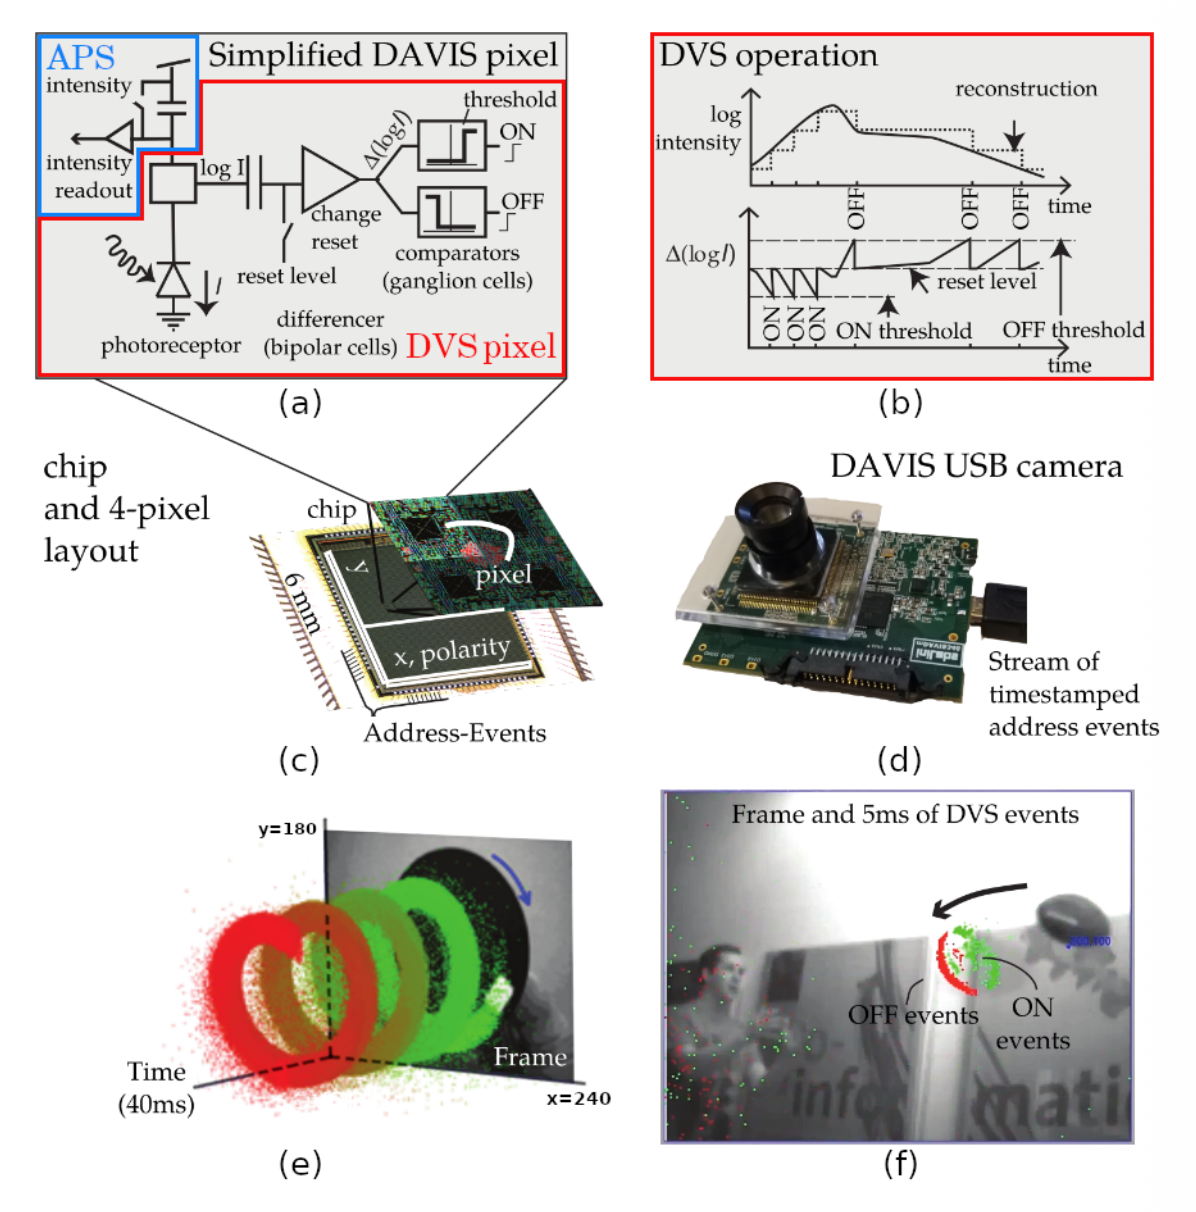
\includegraphics[width=0.75\textwidth]{images/fig_event_camera_principle.png}
    \caption{Operating principle of a Dynamic Vision Sensor (DVS). Each pixel independently and asynchronously fires an event when the change in log luminance exceeds a contrast threshold $C$, producing a stream of events $(x, y, t, p)$ with microsecond temporal resolution. Adapted from \cite{gallego2020event}.}
    \label{fig:dvs_principle}
\end{figure}




\section{Event Representations for Deep Learning}
A central challenge in applying deep learning to event camera data lies in bridging the gap between the asynchronous, sparse nature of event streams and the dense, regular tensor inputs expected by most neural network architectures. Several event representations have been developed to address this challenge, each embodying different trade-offs between information preservation and computational efficiency. 

The simplest representation is the event frame or event histogram, which accumulates events within a fixed time window into a two-dimensional grid where each pixel takes a value in {+1, 0, -1} based on event polarity \cite{gallego2020event}. While this representation is directly compatible with standard CNN architectures, it discards temporal information within the accumulation window, effectively reducing the event stream to a snapshot that loses the very temporal richness that distinguishes event cameras from conventional sensors. 

Voxel grids, proposed by Zhu et al. \cite{zhu2019unsupervised}, address this limitation by discretising the event stream into a three-dimensional spatio-temporal volume. Events are accumulated into B temporal bins, producing a tensor of dimensions B × H × W that preserves temporal ordering. This representation has been widely adopted in subsequent work, including the Events-to-Video (E2VID) reconstruction framework \cite{rebecq2019e2vid} and various optical flow estimation methods. The number of temporal bins B represents a tuneable parameter balancing temporal resolution against computational cost. 

\begin{figure}[htbp]
    \centering
    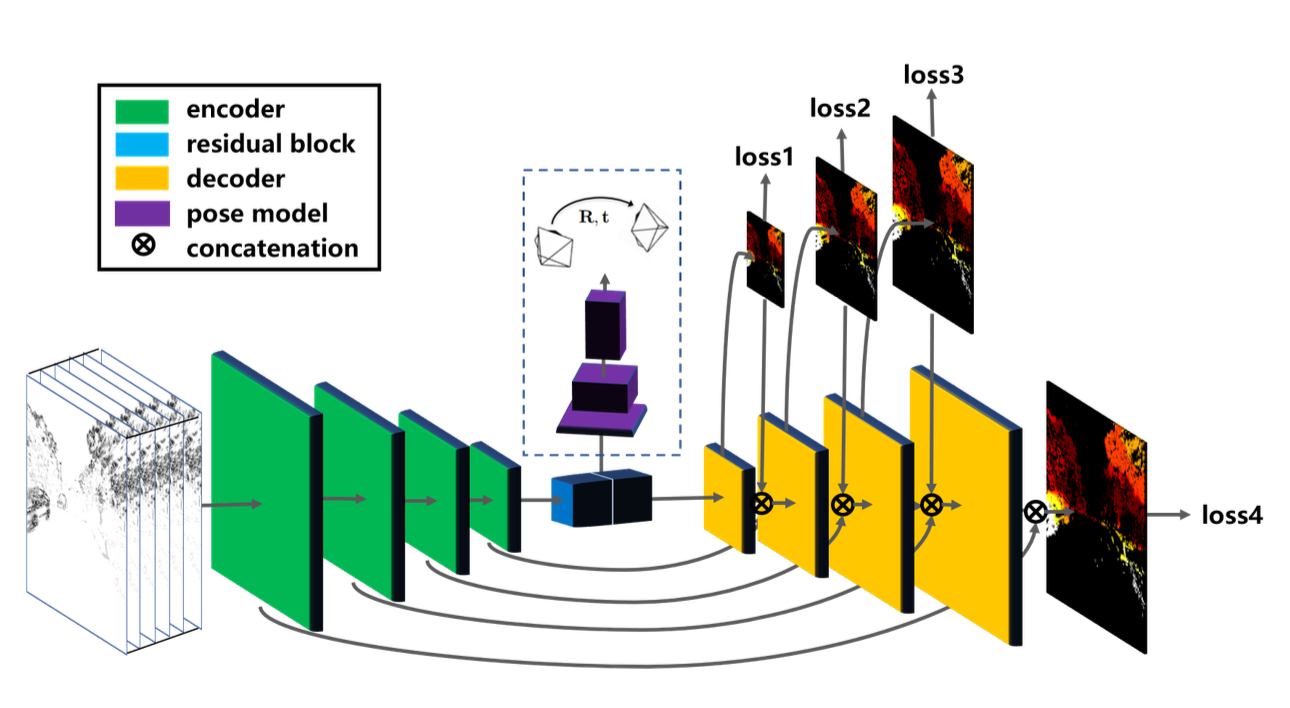
\includegraphics[width=0.75\textwidth]{images/fig_voxel_grid.png}
    \caption{Voxel grid event representation. Events within a fixed time window are accumulated into $B$ temporal bins, producing a tensor of shape $B \times H \times W$ that preserves temporal ordering. Adapted from \cite{zhu2019unsupervised}.}
    \label{fig:voxel_grid}
\end{figure}

Time surfaces, introduced by Lagorce et al. \cite{lagorce2017hots}, offer an alternative encoding where each pixel stores an exponentially decaying function of the time since the last event at that location. This representation naturally encodes recency information and has been extended to Speed-Invariant Time Surfaces (SITS) that normalise for object velocity \cite{manderscheid2019speed}. Time surfaces are particularly effective for feature extraction and pattern recognition tasks, as they encode both spatial structure and temporal dynamics in a compact two-dimensional representation. 

Event Spike Tensors (ESTs), proposed by Gehrig et al. \cite{gehrig2019end}, sample the event stream using learned kernel functions, preserving temporal localisation with minimal information loss. Comparative studies have consistently demonstrated that representations retaining temporal localisation, such as voxel grids and ESTs, outperform simpler aggregation methods like event frames on downstream tasks \cite{gehrig2019end}. This finding underscores the importance of preserving the fine-grained temporal information inherent to event camera outputs. 

More recently, hybrid representations combining multiple channels of information have been explored. For instance, the Temporal Binary Representation packs the presence of events in successive sub-intervals into the bits of a single frame and has improved event-based action recognition \cite{innocenti2021temporal}. The choice of event representation remains an active area of research, with the optimal representation often being task-dependent. 

This work uses the stacked histogram of RVT \cite{gehrig2023recurrent}: per 50-ms window, event counts in ten temporal bins for each of the two polarities (Appendix~\ref{subsec:stacked_hist}). Like a voxel grid it preserves temporal ordering across bins, a property demonstrated to be critical for detection performance \cite{gehrig2019end}, and it is directly compatible with standard CNN and SSM-based backbones. It was not selected by a fresh comparison: it is part of the verified baseline's frozen pipeline (Section~\ref{sec:frozen_pipeline}), and changing it would confound the backbone comparison that is the subject of this thesis. The voxel grid proposed in the Thesis~A plan was therefore not adopted. Time surfaces, although compact, collapse temporal structure into a single 2D map and are less suited to multi-object detection tasks where simultaneous events at different locations must be disambiguated. ESTs offer higher temporal fidelity through learned kernels, but introduce additional parameters and training complexity that is difficult to justify given the computational constraints of onboard UAV deployment. 

Compact multi-channel encodings of this kind have shown promise for action recognition \cite{innocenti2021temporal}, but require careful engineering of the channel structure and have not been validated for detection on the Gen1 automotive dataset used in this work. The bin count $B = 10$ is that of the RVT preprocessing \cite{gehrig2023recurrent}, inherited with the rest of the frozen pipeline. 

\section{Deep Learning for Event-Based Object Detection}
Object detection from event camera data has attracted growing research attention \cite{zheng2023deep}. This review groups the approaches into four paradigms: frame-conversion methods that adapt standard detectors, spiking neural network (SNN) approaches, graph neural network (GNN) methods, and recurrent architectures that process events sequentially. 

\subsection{Frame-Conversion Approaches}
The most straightforward approach to event-based object detection converts event streams into frame-like representations and applies established detection architectures such as YOLO, SSD, or Faster R-CNN. Iacono et al. \cite{iacono2018towards} demonstrated on the iCub humanoid robot that event histograms can be processed by standard object detectors with reasonable accuracy, bootstrapping the event-based annotations from mature frame-based detectors. While this approach benefits from the maturity and optimisation of frame-based detection pipelines, it fundamentally fails to exploit the temporal continuity of the event stream, treating each accumulated frame independently. Furthermore, the frame accumulation step introduces latency that partially negates the low-latency advantage of event cameras. 

Large-scale automotive benchmarks followed: the Gen1 dataset of de Tournemire et al. \cite{detournemire2020large} and the 1Mpx dataset of Perot et al. \cite{perot2020learning}. Perot et al.'s detector, RED, already moves beyond per-window processing: ConvLSTM layers carry information across windows, and a temporal-consistency loss stabilises the predictions over time \cite{perot2020learning}. It belongs with the recurrent architectures discussed below.

\subsection{Spiking Neural Networks}
Spiking neural networks (SNNs) represent a bio-inspired approach that is architecturally well-matched to the asynchronous, binary nature of event camera outputs. In SNNs, information is encoded as discrete spikes rather than continuous activations, enabling highly energy-efficient computation on neuromorphic hardware \cite{roy2019towards}. The DT-LIF (Dual-Threshold Leaky Integrate-and-Fire) neuron model combined with the SSD detection framework, as proposed by Zhou et al. \cite{zhou2023dtlif}, demonstrated that SNNs can perform object detection from event data with significantly lower energy consumption than conventional neural networks. The dual-threshold mechanism improves the neuron's ability to encode temporal patterns by introducing separate thresholds for excitation and inhibition. 

More recently, the Hybrid Spiking Vision Transformer (HsVT) \cite{xu2025hybrid} has integrated spatial feature extraction with temporal spike-based processing, achieving competitive performance with fewer parameters and lower energy consumption than equivalent artificial neural networks. The key advantage of SNN-based detection for micro UAV applications lies in the potential for deployment on neuromorphic processors such as Intel's Loihi or SynSense's Speck chip, which offer orders-of-magnitude improvements in power efficiency compared to conventional GPUs \cite{synsense2026speck}. SNN training is complicated by the non-differentiability of spike generation, and for years spiking detectors lagged behind conventional architectures in accuracy; on Gen1 the most recent ones have closed that gap (Section~\ref{sec:snn_detection}). 

\subsection{Graph Neural Networks}
An alternative paradigm models the event stream as a spatio-temporal graph, where individual events serve as nodes connected to their spatial and temporal neighbours. Graph neural networks (GNNs) can then extract features from this naturally sparse representation without requiring conversion to dense tensors \cite{bi2019graph}. The Asynchronous Event-based GNN (AEGNN) framework \cite{schaefer2022aegnn} demonstrated that graph-based processing preserves the asynchronous nature of events while enabling efficient feature extraction through graph convolutions and pooling operations. The primary advantage of GNN approaches is their ability to process events at their native resolution without temporal binning, potentially preserving more information than frame-based methods. However, the irregular memory access patterns of graph operations can be challenging to optimise on conventional hardware, and scalability to high event rates remains an open problem. 

\subsection{Recurrent Architectures}
Recurrent neural networks (RNNs), particularly convolutional LSTMs and GRUs, have been widely applied to sequential event processing. Recurrent architectures naturally accumulate temporal context across event windows, making them well-suited for tasks requiring temporal reasoning \cite{rebecq2019e2vid}, \cite{cannici2019attention}. The E2VID framework \cite{rebecq2019e2vid}, while primarily targeting video reconstruction, demonstrated that a recurrent UNet encoder-decoder can effectively process temporal sequences of event representations. Detection frameworks have adopted recurrent feature extractors to build temporal context, from the ConvLSTM-based RED \cite{perot2020learning} to RVT \cite{gehrig2023recurrent}. 

The principal limitation of recurrent approaches for deployment on micro UAVs is their sequential processing requirement, which limits parallelisation and can create computational bottlenecks. Additionally, RNNs are known to struggle with very long temporal dependencies due to vanishing gradient problems, though gated variants partially mitigate this issue. Zubic et al. \cite{zubic2024state} report that RNN-based event detectors degrade sharply when deployed at inference frequencies other than their training frequency, a limitation that matters for the variable-rate nature of event camera data. 

\section{State Space Models: Architecture and Evolution}
State Space Models (SSMs) have recently emerged as a powerful class of sequence models that address many of the computational limitations of transformers and recurrent networks \cite{gu2022efficiently}. Rooted in control theory, SSMs model the relationship between an input sequence $u(t)$ and an output sequence $y(t)$ through a latent state $h(t)$ governed by a continuous-time linear dynamical system:

\begin{align}
    h'(t) &= Ah(t) + Bu(t) \\
    y(t) &= Ch(t) + Du(t)
\end{align}

where $A, B, C$, and $D$ are learnable parameter matrices \cite{gu2022efficiently}. This continuous-time formulation can be discretised at arbitrary time steps $\Delta t$ using methods such as the zero-order hold, enabling flexible adaptation to different sampling rates \cite{gu2022efficiently, zubic2024state}. 

The discretisation process transforms the continuous parameters $(A, B)$ into their discrete counterparts $(\overline{A}, \overline{B})$ using the step size $\Delta$:

\begin{equation}
    \overline{A} = \exp(\Delta A), \quad \overline{B} = (\exp(\Delta A) - I)A^{-1}B
\end{equation}

This allows the model to be computed as a linear recurrence, which is significantly more efficient for long sequences than the quadratic complexity of self-attention \cite{gu2023mamba, somvanshi2025from}.

The Structured State Space Sequence Model (S4), proposed by Gu et al. \cite{gu2022efficiently}, represented a breakthrough by introducing a special parameterisation of the state matrix A based on the HiPPO (High-order Polynomial Projection Operator) framework. This parameterisation enables the efficient computation of very long-range dependencies while maintaining linear computational complexity in sequence length. S4 achieved state-of-the-art results on the Long Range Arena benchmark, including the challenging Path-X task with sequence lengths of 16,384, and attained 91\% accuracy on sequential CIFAR-10 \cite{gu2022efficiently}. The S5 variant \cite{smith2023simplified} further simplified the architecture by employing a diagonal state structure with parallel scan mechanisms, eliminating the need for computationally expensive FFT operations while maintaining comparable performance. 

\section{Mamba and Selective State Spaces}
The Mamba architecture, proposed by Gu and Dao \cite{gu2023mamba}, introduced a critical innovation: selective state spaces. Unlike the time-invariant S4 model, Mamba makes the matrices $B$, $C$, and the discretisation step $\Delta$ input-dependent, enabling the model to selectively attend to or ignore different parts of the input sequence based on content \cite{gu2023mamba}. This is achieved by defining these parameters as functions of the input $x_t$:

\begin{align}
    B_t &= \text{Linear}_B(x_t) \\
    C_t &= \text{Linear}_C(x_t) \\
    \Delta_t &= \text{Softplus}(\text{Parameter}_\Delta + \text{Linear}_\Delta(x_t))
\end{align}

This selectivity is analogous to the gating mechanisms in LSTMs and GRUs but operates within the SSM framework while maintaining linear computational complexity \cite{gu2023mamba}. Input-dependent $\Delta_t$ allows for selective retention: a large $\Delta_t$ causes the state to decay rapidly (resetting the memory for irrelevant content), while a small $\Delta_t$ preserves long-range memory \cite{gu2023mamba, zubic2024state}. 

Because the parameters now vary with the input, the model can no longer be computed as a convolution. Mamba instead uses a hardware-aware algorithm that combines a parallel scan, kernel fusion and recomputation, giving about 5$\times$ higher inference throughput than Transformers of similar size while matching their quality in language modelling \cite{gu2023mamba}. Its successor, Mamba-2, recasts the selective scan through state-space duality and runs its core layer 2--8$\times$ faster than Mamba's \cite{dao2024transformers}. Such efficiencies are relevant to the size, weight, and power (SWaP) constraints of micro-UAV platforms.

\begin{figure}[htbp]
    \centering
    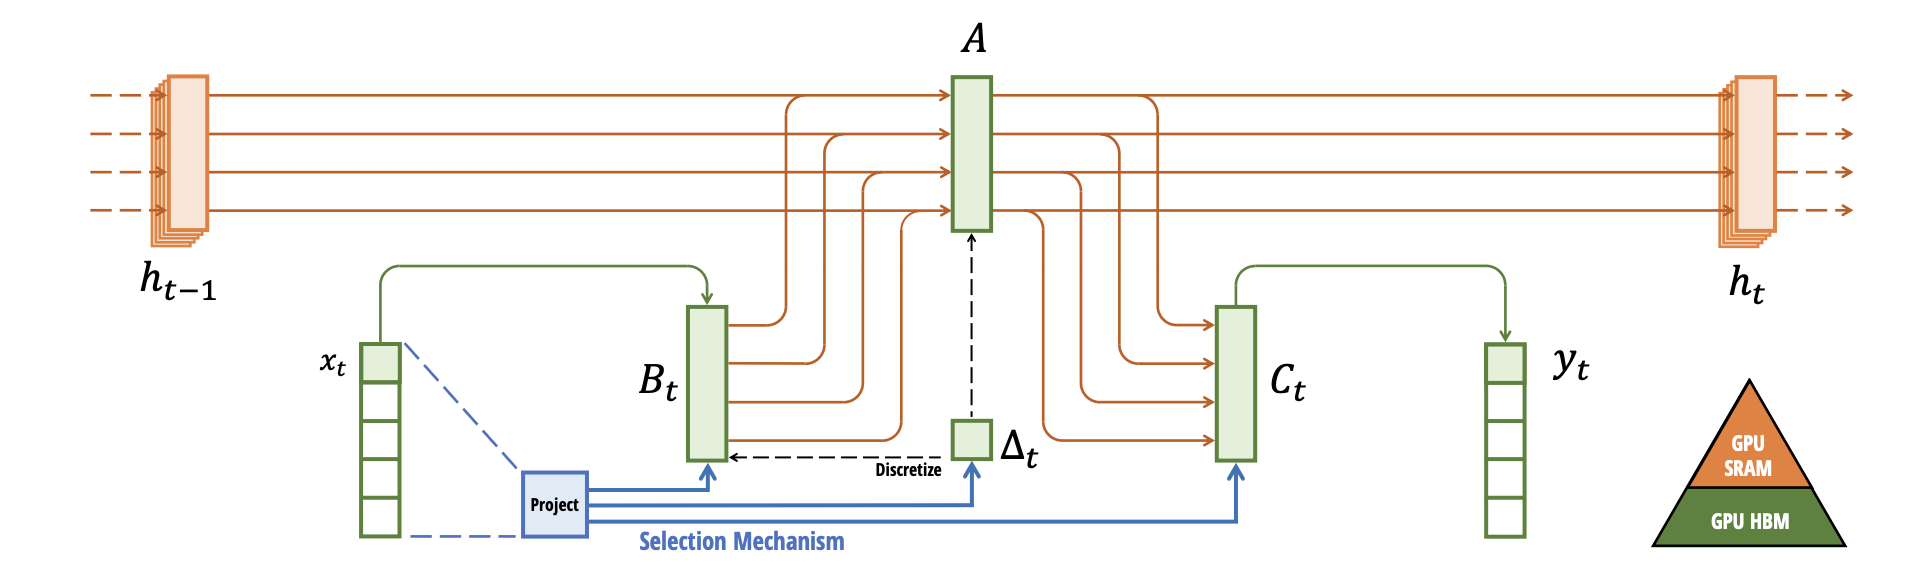
\includegraphics[width=0.85\textwidth]{images/fig_mamba_architecture.png}
    \caption{The Mamba selective state space model architecture. Input-dependent parameters $\Delta_t$, $B_t$, and $C_t$ are computed as functions of the input $x_t$, enabling content-aware selective retention of long-range temporal context while maintaining linear computational complexity. Adapted from \cite{gu2023mamba}.}
    \label{fig:mamba_arch}
\end{figure}

The extension of SSMs to vision tasks has proceeded rapidly. Vision Mamba (Vim) \cite{zhu2024vision} proposed a vision backbone employing bidirectional Mamba blocks with position embeddings, achieving 2.8× faster inference than the DeiT transformer on ImageNet while using 86.8\% less GPU memory for high-resolution image processing. VMamba \cite{liu2024vmamba} introduced Visual State-Space (VSS) blocks with a 2D Selective Scan (SS2D) module that traverses image patches along multiple scan paths to capture two-dimensional spatial relationships. PlainMamba \cite{yang2024plainmamba} further explored non-hierarchical Mamba structures for visual recognition. These vision SSMs consistently demonstrate that the linear complexity of state space models can be leveraged for visual tasks without sacrificing the representational capacity needed for accurate perception. 

The computational advantages of SSMs are particularly relevant for micro UAV applications. The O(n) complexity of SSMs, compared to the O(n²) complexity of transformers, directly translates to reduced inference time and memory consumption. Furthermore, the continuous-time formulation of SSMs allows deployment at variable time scales without retraining, a property that Zubic et al. \cite{zubic2024state} report to be advantageous for event camera data, where the effective data rate varies with scene dynamics. A comprehensive survey by Somvanshi et al. \cite{somvanshi2025from} has catalogued the rapid evolution from S4 to Mamba and its variants, documenting the expanding application of SSMs across vision, language, and multi-modal tasks. 

\section{State Space Models for Event Camera Data}
The intersection of SSMs and event-based vision is a nascent but rapidly developing area. Zubic et al. \cite{zubic2024state} presented the first systematic investigation of SSMs for event camera data, published at CVPR 2024. Their work identified a fundamental limitation of existing deep learning approaches to event data: when trained at one temporal resolution (i.e., a specific ratio between the number of events and the number of forward passes of the network), models based on CNNs, RNNs, and transformers all exhibit significant performance degradation when deployed at different temporal resolutions. This is particularly problematic for event cameras, where the event rate naturally varies with scene dynamics. 

Zubic et al. \cite{zubic2024state} argued that SSMs, viewed as linear time-invariant (LTI) continuous-time systems, can be discretised at arbitrary step sizes without retraining. By rescaling a learnable timescale parameter by the ratio between training and inference frequencies, they report that their SSM-based models maintained performance across a range of deployment frequencies with minimal degradation (3.76 mAP drop versus >20 mAP for RNNs and transformers at higher frequencies). Furthermore, the SSM approach achieved 33\% faster training compared to equivalent recurrent models. If these results hold, SSMs are architecturally well suited to the temporal characteristics of event camera data; Section~\ref{subsec:f2} tests the reported compensation under the released checkpoint and code. 

The most influential baseline for event-based object detection is the Recurrent Vision Transformer (RVT) introduced by Gehrig and Scaramuzza \cite{gehrig2023recurrent}. RVT employs a four-stage hierarchical backbone combining convolutional priors with local and dilated global self-attention, using a ConvLSTM to carry hidden state across consecutive 50~ms windows \cite{gehrig2023recurrent}. A Feature Pyramid Network (FPN) and YOLOX detection head complete the pipeline \cite{gehrig2023recurrent}. 

RVT achieved $47.2$~mAP on the Gen1 automotive dataset with an inference latency below 12~ms, a five-fold reduction compared to prior art \cite{gehrig2023recurrent}. All subsequent SSM-based methods, including those explored in this work, benchmark against RVT, making it the de facto reference architecture for this thesis \cite{gehrig2023recurrent, zubic2024state, yang2025smamba}.

Zubic et al. \cite{zubic2024state}, described above, apply SSMs directly within the RVT framework for event-based object detection, achieving 47.71 mAP on Gen1 with S5 layers replacing the ConvLSTM. Critically, the SSM is used purely for inter-frame temporal aggregation; spatial feature extraction remains handled by Transformer attention blocks. The SSM variant employed is S5, a fixed-parameter (non-selective) model whose transition matrices do not depend on the input. 

Most recently, SMamba \cite{yang2025smamba} (AAAI 2025) advances the state of the art on Gen1 to 50.4 mAP by replacing the spatial Transformer stages of RVT with a Sparse Selective Mamba (S6) backbone. A Spatio-Temporal Continuity Assessment (STCA) module identifies informative tokens and discards noisy or inactive patches before the Mamba scan, reducing FLOPs by 23\% while improving accuracy. Inter-frame temporal context is still provided by a ConvLSTM, not Mamba. SMamba thus shows that a selective Mamba can replace attention for spatial feature extraction in event-based detection while reducing computation. 

Despite this progress, a consistent pattern emerges across the top-performing methods: each keeps inter-frame recurrence (an LSTM or SSM state carried across consecutive windows) and multi-scale FPN detection, and each changes several components of the RVT backbone at once. No prior work has compared a convolutional and a state-space spatial mixer under an otherwise identical backbone, temporal model and training pipeline. That controlled comparison, with a selective (Mamba) temporal recurrence in both models, is the primary architectural contribution of this thesis. The application of SSM-based event detection to micro-UAV platforms with SWaP constraints has no prior demonstration either, and remains outside the evaluation of this thesis (Section~\ref{sec:scope}).

\section{Event-Based Vision for UAV Navigation and Obstacle Avoidance}
The application of event cameras to UAV navigation has been an active area of research, driven by the sensor's inherent advantages for high-speed, low-latency perception. Pioneering work on event-based visual-inertial odometry by Rebecq et al. \cite{rebecq2017real} demonstrated that event cameras could provide accurate ego-motion estimation, a fundamental capability for UAV localisation. Their approach tracked features in motion-compensated event frames and fused them with inertial measurements in a keyframe-based nonlinear optimisation to estimate the 6-DOF pose, remaining robust under rapid motion and high dynamic range. 

Vidal et al. \cite{vidal2018ultimate} extended this work by fusing events, standard frames and inertial measurements in a single state-estimation pipeline (Ultimate SLAM). The fusion improved accuracy by 130\,\% over an events-only and by 85\,\% over a frames-only visual-inertial pipeline, and remained reliable in high-speed and high-dynamic-range scenes, including on a flying quadrotor. 

Falanga et al. \cite{falanga2020dynamic} presented a seminal contribution in event-based obstacle avoidance for quadrotors, building on their analysis of how perception latency limits the safe speed of a sense-and-avoid system \cite{falanga2019fast}. Their approach performed motion segmentation on the event stream to identify independently moving objects, then computed time-to-contact estimates to trigger avoidance manoeuvres. The system achieved an overall processing latency of approximately 3.5 milliseconds, enabling the quadrotor to avoid obstacles at relative speeds up to 10 m/s. Critically, their work demonstrated that event cameras could enable reactive obstacle avoidance at speeds far beyond the capabilities of frame-based perception systems, where the minimum achievable latency is bounded by the frame period (about 17--33~ms at 30--60 frames per second). 

Sanket et al. \cite{sanket2020evdodgenet} proposed EVDodge, an event-based dodging system tested on UAV platforms. Their approach demonstrated real-time obstacle avoidance using purely event-based perception, showing that the high temporal resolution of event cameras could be directly translated into improved avoidance performance. The system was validated both in simulation and on physical quadrotor platforms, confirming the practical feasibility of event-based avoidance systems. 

More recent work has explored bio-inspired processing pipelines for event-based UAV obstacle avoidance. Xu et al. \cite{li2024taming} proposed BioDrone, which processes stereo event cameras with a chiasm-inspired pipeline for fast event filtering and obstacle detection and a lateral-geniculate-nucleus-inspired matching algorithm for obstacle localisation, deployed on an FPGA through software--hardware co-design, and reported an obstacle detection rate of 96.1\%. Such co-designed pipelines are particularly relevant for micro UAVs, where the power budget is a primary constraint. 

Despite these advances, each of the surveyed approaches has notable limitations. The visual odometry and motion segmentation methods of Rebecq et al.\ \cite{rebecq2017real} and Falanga et al.\ \cite{falanga2020dynamic} use handcrafted features and geometric rules rather than learned representations, which limits how well they generalise to new environments. EVDodge \cite{sanket2020evdodgenet}, while shown to work on real hardware, uses a relatively shallow network that has not been tested under challenging conditions such as cluttered scenes or rapidly changing lighting. The bio-inspired pipeline of Xu et al.\ \cite{li2024taming} is attractive for its low latency, but relies on a co-designed FPGA implementation and hand-designed filtering and matching stages rather than the learned spatial features required for general object detection. Most importantly, none of these methods combine learned deep spatial features with a temporal model that can handle variable event rates, the core gap that this thesis addresses through its SSM-based detection architecture. 

\section{Contrast Maximisation and Motion Estimation from Events}
Gallego et al. \cite{gallego2018unifying} proposed a unifying contrast maximisation framework for event-based vision that provides a principled approach to estimating motion, depth, and optical flow from events. The core idea is to warp events according to a candidate motion model and measure the contrast (sharpness) of the resulting warped event image; the motion parameters that maximise contrast correspond to the true motion. This framework elegantly handles the data association problem inherent in event-based motion estimation without requiring explicit feature matching or appearance information. 

The contrast maximisation principle has been extended and refined by subsequent work. Shiba et al. \cite{shiba2024secrets} applied it to dense optical flow, depth, and ego-motion estimation, introducing multi-scale approaches to improve convergence and better handle occlusions. Self-supervised learning-based optical flow methods, such as EV-FlowNet \cite{zhu2018evflownet}, have also been developed, using photometric losses as supervisory signals to learn event-to-flow mappings without requiring ground truth annotations. These motion estimation capabilities are directly relevant to obstacle avoidance, as optical flow and time-to-contact can be used to identify and respond to approaching obstacles.

\section{Event Camera Datasets and Benchmarks}
The availability of standardised datasets has been instrumental in advancing event-based vision research. Several benchmark datasets are relevant to the object detection and navigation tasks considered in this thesis. 

The DSEC dataset \cite{gehrig2021dsec}, developed at the University of Zurich, provides high-resolution stereo event camera data captured using Prophesee Gen3.1 sensors with a 60 cm baseline, complemented by global shutter colour cameras and LiDAR ground truth. DSEC covers a range of driving scenarios under both favourable and challenging illumination conditions, making it a valuable benchmark for event-based depth estimation and optical flow. 

The MVSEC (Multi Vehicle Stereo Event Camera) dataset \cite{zhu2018multivehicle} uses DAVIS346B stereo pairs with a 10 cm baseline, providing synchronised event, frame, IMU, and LiDAR data. MVSEC includes sequences from indoor flying, outdoor driving, and motorcycle scenarios, offering diverse conditions for evaluating perception algorithms. 

For object detection specifically, the Gen1 \cite{detournemire2020large} and 1Mpx \cite{perot2020learning} datasets provide large-scale automotive event recordings from Prophesee cameras with bounding-box annotations: cars and pedestrians in Gen1, and pedestrians, two-wheelers and cars in 1Mpx. The N-Caltech101 dataset \cite{orchard2015converting} provides an event camera version of the Caltech101 classification benchmark, created by displaying images on a monitor in front of a DVS camera executing saccadic movements. While primarily a classification benchmark, N-Caltech101 has been widely used for evaluating event representation and feature extraction methods. 

A significant gap exists in available datasets for UAV-specific scenarios. Most event camera datasets target automotive applications, and there are limited publicly available datasets that capture the specific challenges of micro UAV navigation: rapid ego-motion, indoor environments, small obstacles, and the particular motion patterns characteristic of rotary-wing flight. Addressing this dataset gap remains an open challenge for UAV-specific event-based perception research. For the purposes of this thesis, the primary evaluation is conducted on the Gen1 automotive dataset, which provides a well-established benchmark for detection performance. Obstacle avoidance is treated as a motivating application rather than a directly evaluated system; the trained detection model represents the core perceptual component that such a system would require. Extension to UAV-specific scenarios, potentially through synthetic data generation in open-source simulators such as Gazebo with event camera emulation, is identified as a direction for future work subject to hardware and time constraints. 

\section{Computational Constraints and Obstacle Avoidance for Micro UAVs}
Micro UAVs in the sub-250 gram class face severe SWaP constraints that fundamentally shape the design of onboard perception systems. Typical computational platforms for nano- and micro-UAVs are milliwatt-class microcontrollers and parallel ultra-low-power processors, on which even a compact navigation network runs at only about 9--13 frames per second \cite{niculescu2021improving}; they are orders of magnitude less capable than the GPU-equipped systems used to train and evaluate most deep learning models. This disparity between training and deployment hardware necessitates either highly efficient model architectures, hardware acceleration, or offloading computation to a ground station at the cost of communication latency. 

Several approaches to obstacle avoidance on resource-constrained platforms have been explored. Traditional methods based on optical flow divergence, time-to-contact estimation or event-based motion segmentation provide computationally lightweight avoidance capabilities but lack the ability to classify specific obstacles \cite{decroon2016monocular, falanga2020dynamic}. Model predictive control (MPC) approaches can generate optimal avoidance trajectories but require real-time environmental perception as input. Cooperative approaches, where a less-equipped micro UAV receives guidance from a sensor-rich companion \cite{pritzl2024drones}, offer a pragmatic solution but introduce communication dependencies. 

The emergence of neuromorphic processing hardware offers a potential path to efficient onboard perception. The SynSense Speck chip \cite{synsense2026speck} integrates a dynamic vision sensor with a fully asynchronous spiking neural network processor, achieving real-time event processing with idle power consumption below 1 mW. Similarly, Intel's Loihi processors support on-chip learning and efficient SNN inference \cite{davies2021advancing}, and Loihi~2 adds programmable neuron models and graded spikes \cite{orchard2021efficient}. These platforms are particularly well-suited to processing event camera data, as they natively handle the sparse, asynchronous data format. However, the software ecosystem for neuromorphic processors remains immature compared to conventional deep learning frameworks, and mapping complex detection architectures onto neuromorphic hardware remains an active research challenge. 

The linear complexity and inherent efficiency of SSM-based architectures position them as strong candidates for deployment on the limited computational resources available on micro UAVs. Unlike transformer-based models, whose memory and computation grow quadratically with sequence length, SSMs process long event sequences with a fixed-size recurrent state, although that state can be large (Section~\ref{sec:efficiency}). Combined with model compression techniques such as quantisation and pruning, SSM architectures may enable real-time object detection on platforms that cannot support transformer or large CNN inference. 

\section{Identification of Research Gaps}
\label{sec:gaps_thesisA}
The preceding review reveals several interconnected research gaps that this thesis aims to address: 

Gap 1: Pure selective Mamba for event-based object detection. Existing SSM-based detection methods integrate SSM layers into Transformer backbones \cite{zubic2024state} or employ selective Mamba within sparse-attention hybrid frameworks \cite{yang2025smamba}. In both cases, inter-frame recurrence is maintained via ConvLSTM or SSM hidden state passed across consecutive windows. No prior work has evaluated a fully recurrence-free, convolutional-free selective Mamba architecture for event-based detection, nor conducted a controlled ablation comparing a CNN-SSM hybrid against a pure SSM model under identical loss functions, detection heads, and training protocols. Such a comparison is required to isolate the contribution of the spatial feature extractor from all other architectural variables. 

Gap 2: Integrated detection and avoidance for micro UAVs. Existing event-based UAV obstacle avoidance systems \cite{falanga2020dynamic, sanket2020evdodgenet} predominantly employ reactive strategies based on optical flow or motion segmentation, without explicit object detection. Conversely, event-based detection methods \cite{perot2020learning,gehrig2023recurrent} have been evaluated primarily on automotive benchmarks. An integrated system that combines SSM-based object detection with obstacle avoidance control, specifically designed for micro UAV deployment, has not been demonstrated. 

Gap 3: Computational efficiency benchmarking for onboard deployment. While the theoretical computational advantages of SSMs over transformers and RNNs are well-established, systematic benchmarking of SSM inference latency, memory consumption, and energy usage on the constrained hardware platforms typical of micro UAVs has not been conducted. Understanding the practical deployment characteristics of SSM-based detection models is essential for validating their suitability for this application domain. 

Gap 4: Variable-rate event processing for obstacle avoidance. The unique ability of SSMs to generalise across temporal resolutions \cite{zubic2024state} has not been exploited in the context of obstacle avoidance, where the event rate varies dramatically with UAV speed and scene complexity. An adaptive processing framework that adjusts its temporal resolution based on event rate while maintaining detection performance could significantly improve both efficiency and robustness. 

As registered in Thesis~A, these gaps defined the research space as developing and evaluating SSM-based architectures for event-based object detection and obstacle avoidance on micro UAVs, with a focus on computational efficiency, temporal adaptability and practical deployability. Section~\ref{sec:gaps_revisited} revises them after the scope change. 


% --- Chapter 3: Methodology ---


\section{Spiking Neural Networks for Event-Based Detection}
\label{sec:snn_detection}
Directly-trained spiking neural networks (SNNs) are an established family on this benchmark and the
comparison class for the neuromorphic strand of this thesis. They are trained with surrogate
gradients~\cite{neftci2019surrogate}: the non-differentiable spike function is kept in the forward pass
and replaced by a smooth surrogate derivative in the backward pass, which makes back-propagation through
time applicable to networks of spiking neurons. Table~\ref{tab:snn_landscape} places the spiking detectors
reported on Gen1 against the non-spiking models of this thesis.

\begin{table}[htbp]
\centering
\small
\caption{Object detection on Prophesee Gen1, COCO mAP@[0.50:0.95] on the test split. Ranges span the
reported model sizes. $T\times D$: timesteps $\times$ virtual timesteps of integer-valued training
($D=1$: binary spikes throughout). SpikeDet is a preprint (version 5, 2026); its first version, under
the title SpikSSD, reported 40.8.}
\label{tab:snn_landscape}
\begin{tabularx}{\textwidth}{@{}l>{\raggedright\arraybackslash}Xccl@{}}
\toprule
\textbf{Model} & \textbf{Type} & \textbf{$T\times D$} & \textbf{mAP} & \textbf{Venue} \\
\midrule
RVT \cite{gehrig2023recurrent}        & ANN (attention, ConvLSTM) & --- & 47.2 & CVPR 2023 \\
S5-RVT \cite{zubic2024state}          & ANN (attention, S5)       & --- & 47.7 & CVPR 2024 \\
SMamba \cite{yang2025smamba}          & ANN (sparse Mamba, ConvLSTM) & --- & 50.4 & AAAI 2025 \\
EventSSM (this work)                  & ANN (convolution, Mamba-2) & --- & 46.2 & --- \\
PureSSM (this work)                   & ANN (BiMamba, Mamba-2)    & --- & 46.4 & --- \\
\midrule
HsVT \cite{xu2025hybrid}              & hybrid (spiking temporal block) & --- & 44.9--47.8 & ICML 2025 \\
SpikeDet \cite{fan2025spikedet}       & SNN, integer-valued       & $5\times1$, $4\times2$ & 46.5--47.6 & preprint \\
EAS-SNN \cite{wang2024eas}            & SNN, recurrent            & $3$ & 37.2--40.9 & ECCV 2024 \\
SpikeYOLO \cite{luo2024integer}       & SNN, integer-valued       & $5\times1$, $4\times2$ & 38.5--40.4 & ECCV 2024 \\
EMS-YOLO \cite{su2023deep}            & SNN                       & $5$ & 26.7--31.0 & ICCV 2023 \\
\bottomrule
\end{tabularx}
\end{table}

Two observations follow. First, the accuracy gap between spiking and non-spiking detectors on Gen1 has
closed. EMS-YOLO, the first deep directly-trained spiking detector~\cite{su2023deep}, reached 31.0 in 2023,
16.7~mAP below S5-RVT; the strongest recent spiking detectors, SpikeDet~\cite{fan2025spikedet} and
HsVT~\cite{xu2025hybrid}, report 47.6 and 47.8, level with S5-RVT and above the own models of this thesis.
On this benchmark a spiking detector is therefore no longer necessarily a less accurate one, and the case
for the neuromorphic strand rests on energy and deployment rather than accuracy.

Second, the mechanisms behind that progress are identifiable, and both are native to a state-space neuron.
\emph{More information per spike:} SpikeYOLO's I-LIF neuron emits integer values in $\{0,\dots,D\}$ during
training and, at inference, expands each integer into $D$ binary spikes over virtual timesteps, so that
inference remains spike-driven (binary, accumulate-only) while training sees a multi-bit
signal~\cite{luo2024integer}. SpikeDet uses the same integer-valued scheme, and for both detectors the
$4\times2$ configuration, with fewer timesteps each carrying a two-level value, outperforms $5\times1$. \emph{Temporal state:}
EAS-SNN uses recurrent convolutional SNNs with temporal memory as an adaptive event sampler~\cite{wang2024eas},
and HsVT combines LSTM blocks with a spiking temporal feature-extraction block on a MaxViT spatial
backbone~\cite{xu2025hybrid}. HsVT is the closest design point to the spiking model of this thesis: it keeps
spatial processing in non-spiking form and spikes along time. A state-space neuron supplies both mechanisms
by construction, since its state is a carried, multi-valued memory and the graded readout of
Section~\ref{subsec:readout_modes} is the per-neuron analogue of an integer-valued spike. EMS-YOLO and
SpikeYOLO also report an ANN of equivalent architecture, so the overall cost of spiking is known for those
designs; where that cost comes from is not reported.

\section{Spiking State Space Models}
\label{sec:spiking_ssm}
A discretised diagonal state-space model and a leaky integrate-and-fire neuron are the same linear
recurrence with different readouts. Consider one state dimension of a diagonal SSM with decay $a<0$,
input weight $b$, output weight $c$ and step $\Delta$, discretised with a zero-order hold:
\begin{equation}
  h_t = \bar a\, h_{t-1} + \bar b\, u_t, \qquad y_t = c\, h_t, \qquad
  \bar a = e^{\Delta a}, \quad \bar b = \frac{e^{\Delta a}-1}{a}\, b .
  \label{eq:ssm_scalar}
\end{equation}
The discrete LIF neuron of Equations~\eqref{eq:lif_integrate}--\eqref{eq:lif_reset} integrates its input
$x_t$ as $m_t = \beta m_{t-1} + x_t$. With $\beta = \bar a$ and $x_t = \bar b u_t$ the membrane potential
$m_t$ \emph{is} the SSM state $h_t$, and the leak is a discretised decay. The neuron differs in two
respects only. Its readout is a threshold, $s_t = \Theta(m_t - \vartheta)$, instead of a linear map; and its
reset, $m_t \leftarrow m_t - s_t\vartheta$, feeds the output back into the state. The second difference is
the consequential one. Without reset the recurrence is linear and can be evaluated with a parallel scan, as
SSMs are during training; with reset the state depends on its own thresholded past, and the recurrence must
be unrolled sequentially. Much of the spiking-SSM literature consists of ways around that obstacle,
summarised in Table~\ref{tab:spiking_ssm}.

\begin{table}[htbp]
\centering
\small
\caption{Spiking state-space models. All except the last row target one-dimensional sequence tasks.}
\label{tab:spiking_ssm}
\begin{tabularx}{\textwidth}{@{}l>{\raggedright\arraybackslash}X>{\raggedright\arraybackslash}Xl@{}}
\toprule
\textbf{Work} & \textbf{How spiking enters} & \textbf{Parallel training} & \textbf{Task} \\
\midrule
SpikingSSMs \cite{shen2025spikingssms} & spiking neurons with learnable thresholds driven by an S4D-type SSM &
  a small network predicts the after-reset membrane & LRA, WikiText-103 \\
SPikE-SSM \cite{zhong2024spike} & reset-refractory neuron, trainable thresholds & boundary compression of
  the membrane & LRA, WikiText-103 \\
P-SpikeSSM \cite{bal2025p} & spikes sampled stochastically from an SSM-based neuron & sampling replaces
  sequential spike generation & long-range tasks \\
SiLIF \cite{fabre2025silif} & the neuron is a two-state SSM with S4-style parametrisation & --- (surrogate
  gradients through time) & speech \\
Spiking-S4 \cite{du2023spiking} & spiking neurons combined with an S4 model & --- & speech enhancement \\
SpikeMba \cite{li2024spikemba} & spiking saliency detector for proposals; Mamba non-spiking & --- &
  video grounding \\
\midrule
This thesis & LIF readout on the output of a selective (Mamba-2) temporal block & SSM scan unchanged;
  readout unrolled over the clip & event detection \\
\bottomrule
\end{tabularx}
\end{table}

SpikingSSMs~\cite{shen2025spikingssms} train a lightweight surrogate dynamic network to predict the
after-reset membrane potential, which restores parallel training with orders-of-magnitude speed-ups over
iterative unrolling, and report performance competitive with non-spiking SSMs at about 90\,\% network
sparsity. SPikE-SSM~\cite{zhong2024spike} accelerates the same computation by compressing the membrane
dynamics between spike boundaries and adds a reset-refractory neuron with trainable thresholds.
P-SpikeSSM~\cite{bal2025p} avoids sequential spike generation altogether by sampling spikes stochastically
from an SSM-based neuronal model. SiLIF~\cite{fabre2025silif} takes the correspondence of
Equation~\eqref{eq:ssm_scalar} in the other direction: it makes it exact for a two-state adaptive neuron and
gives the neuron an S4-style parametrisation (decays trained in logarithmic form, a learnable per-neuron step,
and a complex-valued variant with oscillatory dynamics), reporting state-of-the-art accuracy among spiking
neuron models on speech. Spiking-S4~\cite{du2023spiking} combines S4 with spiking neurons for speech
enhancement at reduced parameter and FLOP counts.

Two limitations of this literature matter here. First, it targets one-dimensional sequence tasks: long-range
benchmarks, language modelling and speech. Second, it is built on linear time-invariant SSMs (S4, S4D), whose
decay does not depend on the input. The only selective model in Table~\ref{tab:spiking_ssm}, SpikeMba, keeps
Mamba itself non-spiking and uses spikes only for proposal generation~\cite{li2024spikemba}. In a selective
SSM the decay $\bar a_t = e^{\Delta_t a}$ varies with the input at every step. The recurrence is still linear
in the state, so a spiking \emph{readout} placed after the scan, as in this thesis, leaves the scan exact and
parallel; making the selective state itself spike, with a reset inside the scan, would require one of the
parallel-training devices above to be extended to input-dependent decays.

\section{Neuromorphic Hardware and the Deployment Path}
\label{sec:neuromorphic_hw}
Neuromorphic processors execute spiking networks in an event-driven manner: computation and
communication happen only when spikes arrive, so energy scales with activity rather than with the size of
the input~\cite{davies2021advancing}. Two features of Intel's Loihi~2 matter for state-space models.
Its neuron models are programmable in microcode rather than fixed to a LIF primitive, so any small
per-neuron recurrence, including the state update of a diagonal SSM, can be implemented directly; and it
supports graded spikes, which carry an integer payload rather than a single bit~\cite{orchard2021efficient},
the hardware counterpart of integer-valued and graded readouts.

Meyer et al.~\cite{meyer2024diagonal} gave the first implementation of an SSM on neuromorphic hardware,
mapping S4D to Loihi~2. The comparison with an NVIDIA Jetson Orin Nano depends on the processing mode. In
offline, batched, sample-by-sample processing the Jetson performed better; in token-by-token processing,
Loihi~2 consumed about 1000 times less energy, with 75 times lower latency and 75 times higher throughput,
than a recurrent S4D implementation on the Jetson. Token-by-token processing is exactly the regime of a
streaming event camera, which is why this result motivates the neuromorphic strand. It was obtained for a
linear time-invariant SSM on one-dimensional sequence benchmarks; a selective SSM, whose decay must be
recomputed from the input at every step, and a two-dimensional detection backbone remain untested on such
hardware. Other neuromorphic substrates take a different route: SynSense's Speck integrates an event sensor
and a spiking processor on one chip~\cite{synsense2026speck}.

Energy figures for spiking detectors run on GPUs are estimates, not measurements. The convention in the
detection literature is to count synaptic operations and multiply them by a per-operation energy, typically
0.9~pJ for a 32-bit floating-point accumulate against 4.6~pJ for a multiply--accumulate at
45~nm~\cite{horowitz2014computing,su2023deep,luo2024integer}. Such estimates ignore memory access and data
movement, which dominate energy on real hardware, so they rank designs rather than predict silicon
consumption; measured results such as Meyer et al.'s are rare by comparison.

The software path is in transition. Intel archived its Lava framework on 13 May 2026, stated that it will
no longer maintain it, and announced a successor SDK without a public timeline~\cite{intel2026lava}. The
Neuromorphic Intermediate Representation (NIR) defines a common set of computational primitives through
which models can be exchanged between simulators and neuromorphic hardware~\cite{pedersen2024neuromorphic},
and is used in this thesis as the export boundary for that reason.

\section{Research Gaps Revisited}
\label{sec:gaps_revisited}
The gap list of Section~\ref{sec:gaps_thesisA}, carried over from Thesis~A, assumed an integrated
detection-and-avoidance system. After the scope change (Section~\ref{sec:scope_change}) its second gap,
integrated detection and avoidance, is retired; its fourth, variable-rate processing for avoidance,
survives as the rate robustness of the detector alone. Its first gap asked for a recurrence-free,
convolution-free selective Mamba detector. The models built here keep a selective temporal recurrence ---
an asset, as the rate-robustness results show --- and a strided convolutional stem, so that gap is
restated as Gap~A below. Its third gap, benchmarking on constrained hardware, is addressed only in part:
latency, energy and memory are measured for every model, but on a desktop GPU rather than embedded
hardware (Section~\ref{sec:efficiency}). The gaps this thesis addresses are narrower
and better defended than those originally proposed.

\textbf{Gap~A: the isolated effect of the spatial mixer.} Published SSM detectors change several things at
once. S5-RVT replaces the temporal mixer of an attention backbone~\cite{zubic2024state}; SMamba replaces the
spatial attention with a sparse Mamba, adds token selection and keeps a ConvLSTM in
time~\cite{yang2025smamba}. Neither isolates what the spatial mixer itself contributes. This thesis
measures it with two detectors that differ only in that component (Section~\ref{sec:acc_results}).

\textbf{Gap~B: rate robustness under the published artefacts.} The temporal generalisation of SSM detectors
has been attributed to inference-time rescaling of the discretisation step~\cite{zubic2024state}. Whether
the reported high-rate results can be reproduced from the released checkpoint and code, and how the
robustness behaves under a fixed cadence versus a true rate change, had not been examined
(Section~\ref{sec:robustness}).

\textbf{Gap~C: where the cost of spiking comes from.} Spiking detectors have reached the accuracy of
non-spiking ones on Gen1 (Table~\ref{tab:snn_landscape}), and spiking SSMs exist for sequence tasks
(Table~\ref{tab:spiking_ssm}). To the author's knowledge, no surveyed work combines a selective state-space
temporal core with spiking for event-based detection, and none decomposes the cost of spiking into the cost
of the neuron dynamics, of sparsity and of binarisation against a non-spiking twin trained through an
identical pipeline. The three readouts of Section~\ref{subsec:readout_modes}, which share one membrane, are
designed to measure exactly that decomposition (Section~\ref{sec:spiking_results}).


\chapter{Methodology}
\label{ch:method}

\section{The Frozen Pipeline}
\label{sec:frozen_pipeline}
The methodological core of this thesis is that the pipeline around the backbone never changes. Every
model reuses the verified S5-RVT/RVT infrastructure \emph{unmodified} and Hydra-selectable:

\begin{itemize}
  \item \textbf{Input representation:} a 20-channel stacked histogram of shape $(20, 240, 304)$
        (2 polarities $\times$ 10 temporal bins, $\Delta t = 50$\,ms), zero-padded by
        the pipeline to $(20, 256, 320)$.
  \item \textbf{Neck:} YOLO-PAFPN. \textbf{Head:} YOLOX decoupled head.
  \item \textbf{Loss:} binary cross-entropy (classification and objectness) $+$ IoU loss $1-\mathrm{IoU}^2$
        (weight 5) with SimOTA label assignment.
  \item \textbf{Data:} Prophesee Gen1 (cars, pedestrians). \textbf{Evaluation:} the Prophesee/COCO evaluator.
  \item \textbf{Training:} PyTorch Lightning, 400k-step OneCycle schedule, bf16 mixed precision.
\end{itemize}

Because only the backbone changes, and between EventSSM and PureSSM only the \emph{spatial mixer}
changes (with its initialisation: ImageNet weights for the convolutional mixer, none for the state-space
one), the difference between those two models is attributable to that swap. Against the published S5-RVT
baseline the comparison is looser: both mixers of the backbone differ, and the own models were trained
with batch size 4 and bf16 mixed precision rather than 8 and 32-bit (Section~\ref{sec:training}). Figure~\ref{fig:spiking_arch}(a)
shows the shared pipeline and the two mixing axes within a backbone stage.

\begin{figure}[htbp]
    \centering
    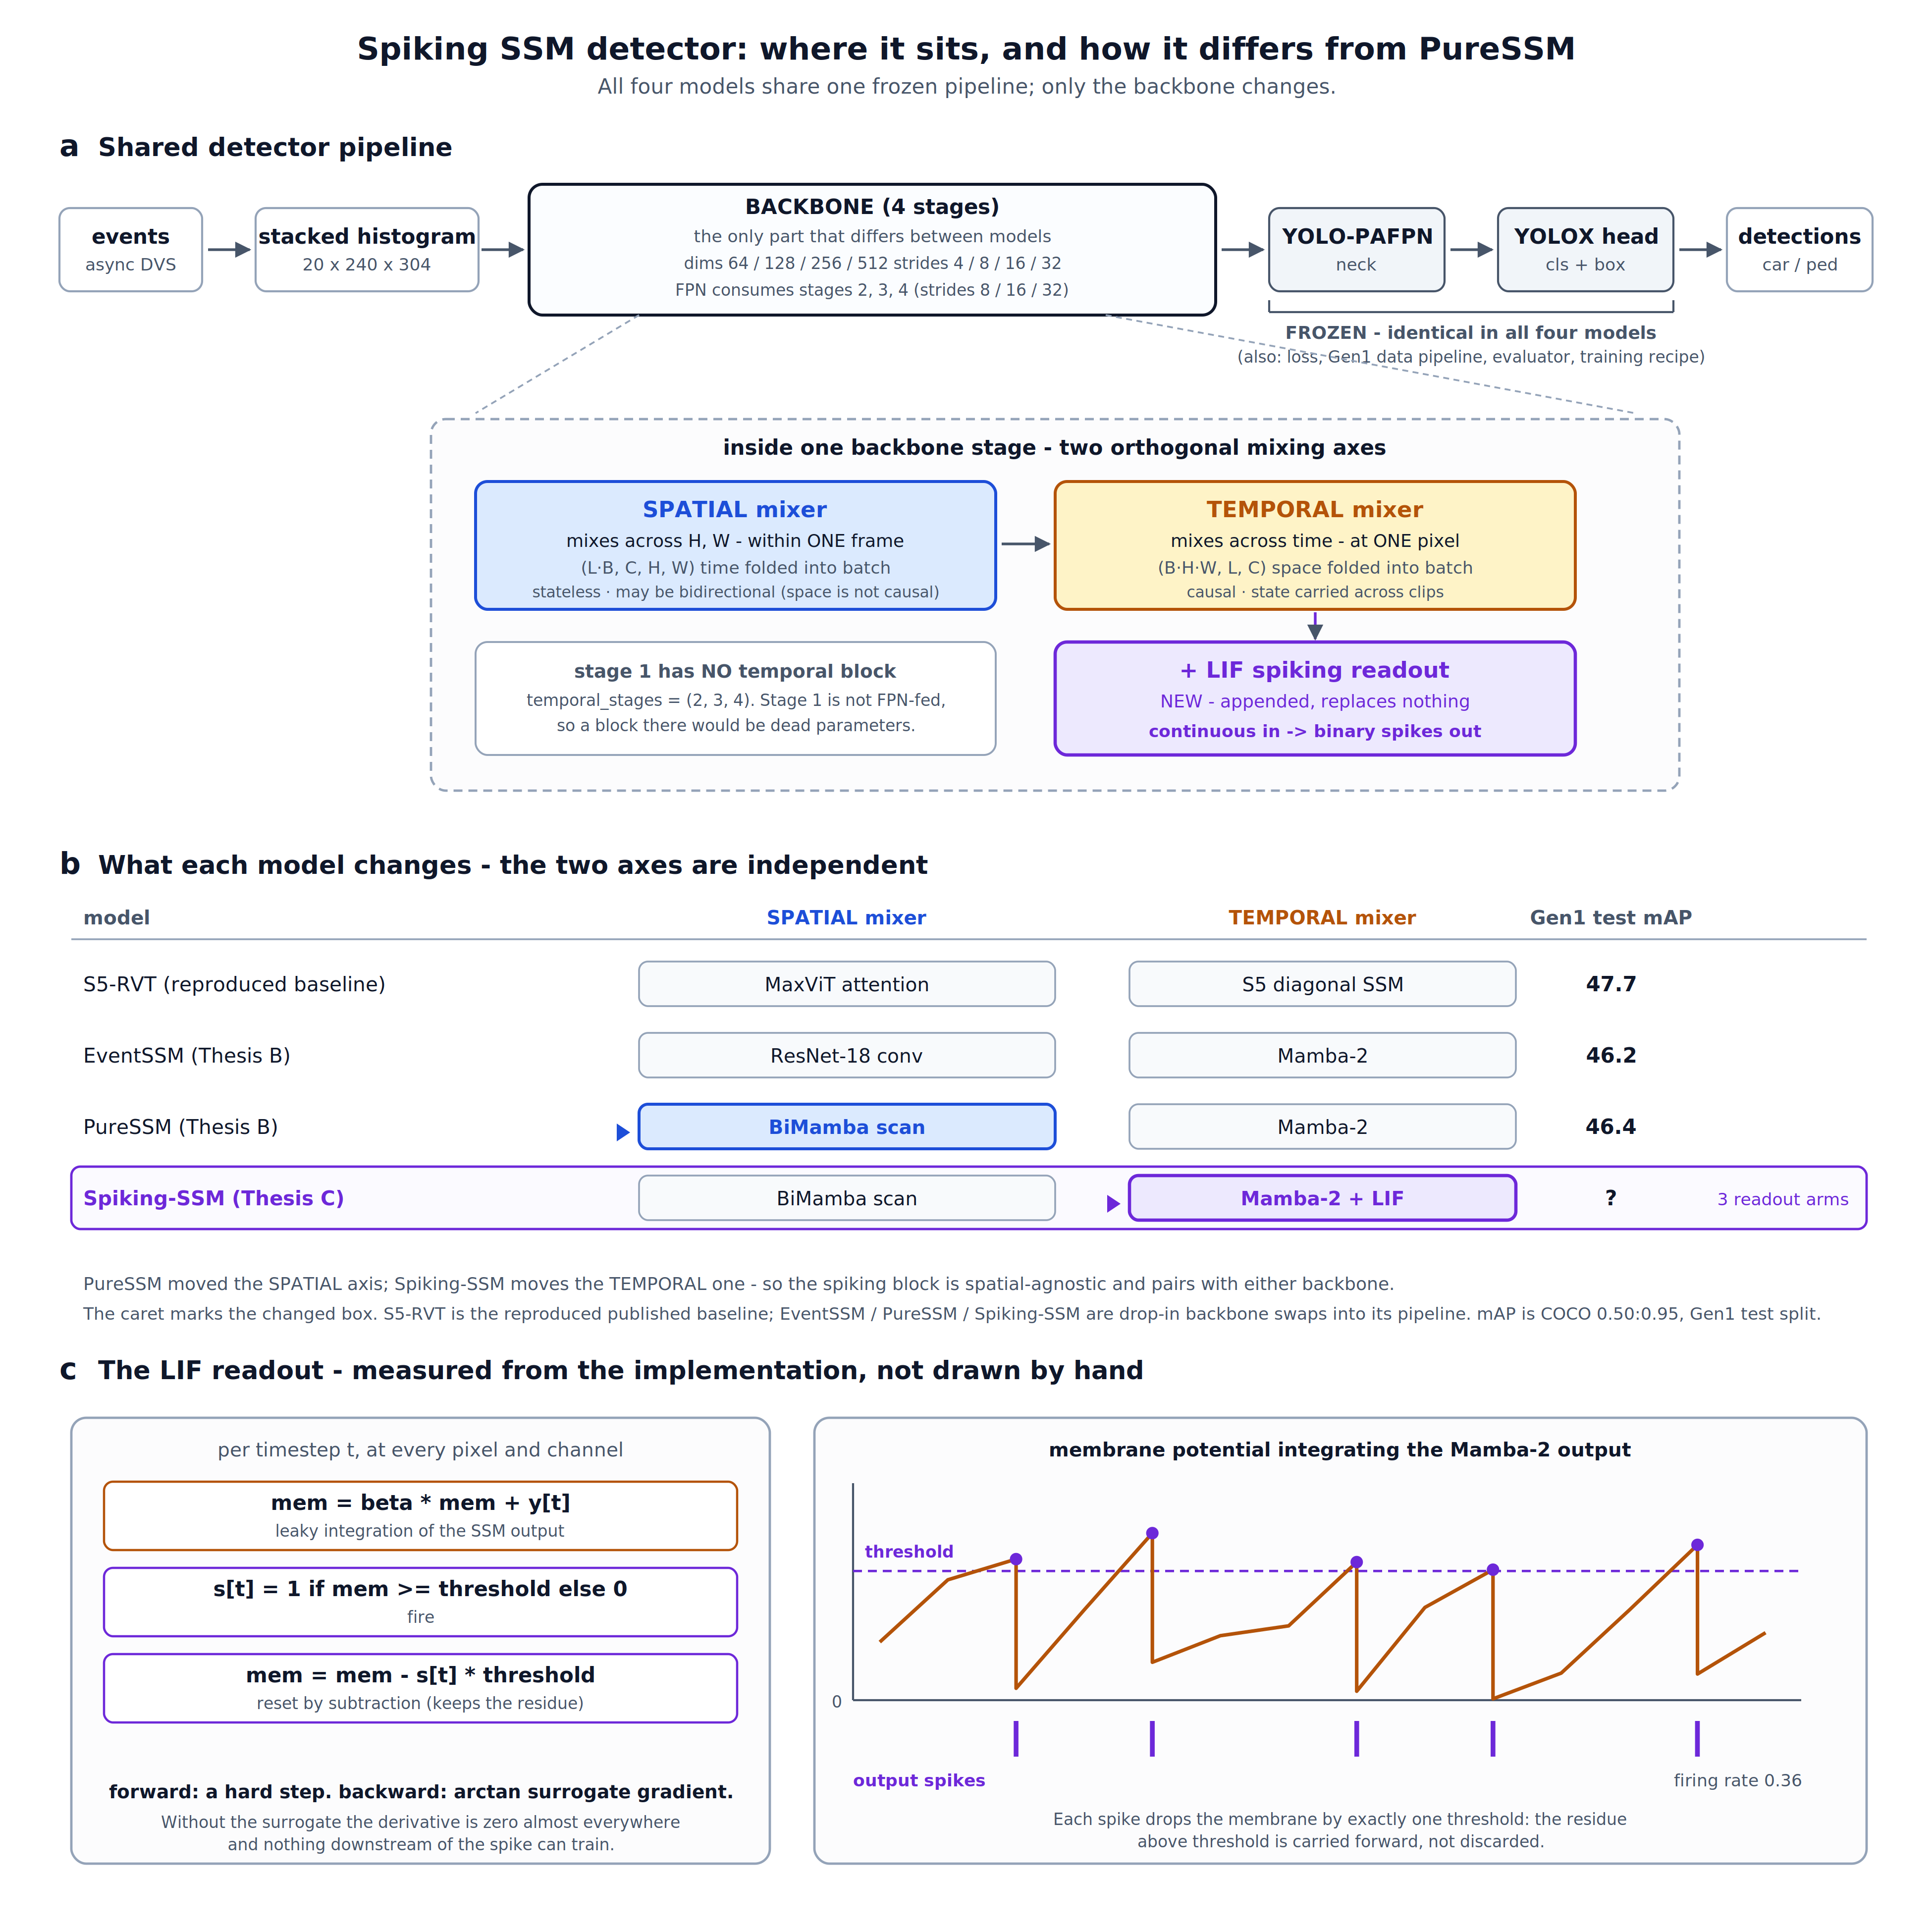
\includegraphics[width=\textwidth]{images/fig_spiking_architecture.png}
    \caption{(a) The shared detector pipeline. The backbone is the only part that differs between
    models; the neck, head, loss, data pipeline and evaluator are frozen. Within a backbone stage
    there are two orthogonal mixing axes: a \emph{spatial} mixer acting within a frame (time folded
    into the batch, stateless) and a \emph{temporal} mixer acting across frames at each pixel (causal,
    state carried across clips). (b) Where each model intervenes: PureSSM changes the spatial axis,
    the spiking model changes the temporal one. (c) The LIF readout; the membrane trace is generated
    by executing the implementation itself rather than drawn by hand.}
    \label{fig:spiking_arch}
\end{figure}

\subsection{The Two Mixing Axes}
\label{subsec:two_axes}
Each backbone stage applies its spatial mixer to every frame independently, with time folded into the
batch dimension, $(L\cdot B, C, H, W)$. It then re-folds to $(B\cdot H\cdot W, L, C)$ and applies its
temporal mixer along the time axis at each spatial location independently. The two axes are therefore
orthogonal, which is what allows them to be varied one at a time. Temporal blocks are instantiated only
for the FPN-consumed stages 2, 3 and 4; stage~1 carries no temporal block, since a block there would
contribute only dead parameters.

The temporal blocks are per-scale \emph{taps} on the spatial pyramid, not links inside it. The pyramid is
evaluated on every frame first; each temporal output then goes to the neck, while the next spatial stage
continues from the per-frame features. This differs from RVT~\cite{gehrig2023recurrent}, where the
recurrent output of each stage is the input of the next, so that deeper stages see temporally integrated
features. Here the deeper spatial stages operate on single frames, and in exchange the whole spatial
pyramid is stateless and can process all frames of a clip in one batched pass. The temporal output
\emph{replaces} the stage features; there is no residual path around the temporal block. The design is
identical in all three own models, so it does not confound their comparison; against the RVT-family
baselines it is one of the architectural differences of the backbone.

\section{The Four Models}
\label{sec:four_models}

\begin{table}[htbp]
\centering
\caption{The four models. For the own models, the component in bold is what changes relative to the row
above; S5-RVT and EventSSM differ in both mixers.}
\label{tab:four_models}
\begin{tabularx}{\textwidth}{@{}lXXX@{}}
\toprule
\textbf{Model} & \textbf{Spatial mixer} & \textbf{Temporal mixer} & \textbf{Role} \\
\midrule
RVT & MaxViT (local + grid attention) & ConvLSTM & Literature baseline \\
S5-RVT & MaxViT & S5 (diagonal SSM) & Reproduced reference \\
EventSSM (this work) & ResNet-18 conv, 3$\to$20-ch adapted, ImageNet-init & Mamba-2 (causal, per-pixel) & CNN--SSM hybrid \\
PureSSM (this work) & \textbf{BiMamba} (bidirectional scan) & Mamba-2 (identical) & Pure state-space detector \\
Spiking-SSM (this work) & BiMamba (identical) & Mamba-2 $+$ \textbf{LIF readout} & Spiking detector \\
\bottomrule
\end{tabularx}
\end{table}

\subsection{EventSSM --- convolutional spatial, state-space temporal}
\label{subsec:eventssm}
\textbf{Spatial mixer.} The spatial pyramid is an ImageNet-initialised ResNet-18~\cite{he2016deep}: a stem
($7\times7$ stride-2 convolution, batch normalisation, ReLU, max-pooling) followed by four residual stages
of widths 64/128/256/512 at strides 4/8/16/32, which on the padded $256\times320$ input produce maps from
$64\times80$ down to $8\times10$. The pretrained first convolution expects three RGB channels. It is
adapted to the 20 histogram channels by \emph{average projection}: the pretrained kernel
$W\in\mathbb{R}^{64\times3\times7\times7}$ is averaged over its input channels, tiled across the 20 new
channels and rescaled,
\begin{equation}
  W'_{:,c} \;=\; \frac{3}{20}\cdot\frac{1}{3}\sum_{k=1}^{3} W_{:,k}, \qquad c = 1,\dots,20,
  \label{eq:avg_projection}
\end{equation}
so that the summed response of each filter to a spatially uniform input equals that of the original, and
the pretrained edge and blob detectors are available to every bin and polarity. All later layers keep
their ImageNet weights.

\textbf{Temporal mixer.} One Mamba-2 layer~\cite{dao2024transformers} acts on each FPN-fed stage
$s\in\{2,3,4\}$ at that stage's width $C_s\in\{128,256,512\}$, with state size $N=64$, expansion factor 2
(so $2C_s/64$ heads of dimension $P=64$) and a causal convolution of width 4. The clip of shape
$(L, B, C_s, h_s, w_s)$ is folded into $B\,h_s w_s$ independent sequences of length $L$, one per spatial
location, and each head $j$ runs the selective recurrence
\begin{align}
  H^{(j)}_t &= \exp\!\big(\Delta^{(j)}_t a^{(j)}\big)\, H^{(j)}_{t-1} + \Delta^{(j)}_t\, x^{(j)}_t B_t^{\top},
  \label{eq:mamba2_state}\\
  y^{(j)}_t &= H^{(j)}_t C_t + D^{(j)} x^{(j)}_t,
  \label{eq:mamba2_out}
\end{align}
where $x^{(j)}_t\in\mathbb{R}^{P}$ is the head's slice of the expanded and causally convolved input,
$H^{(j)}_t\in\mathbb{R}^{P\times N}$ its state, $a^{(j)}<0$ a learned scalar decay,
$\Delta^{(j)}_t=\mathrm{softplus}(\cdot)>0$ an input-dependent step, $B_t, C_t\in\mathbb{R}^{N}$
input-dependent projections shared by all heads, and $D^{(j)}$ a learned skip weight. The heads are
concatenated into $y_t$ and the layer outputs $W_{\mathrm{out}}\,\mathrm{RMSNorm}\big(y_t\odot\mathrm{SiLU}(z_t)\big)$,
with $z_t$ a gate projected from the input. In contrast to S4 and S5, the decay
$\exp(\Delta_t a)$ depends on the input; Section~\ref{sec:robustness} examines what that selectivity does
when the event rate changes.

\textbf{State.} Each temporal layer carries two tensors across clips for every spatial location: the
last three pre-convolution inputs (the left context of the causal convolution) and the head states
$\{H^{(j)}\}$. They are stored batch-major, which lets RVT's existing state container detach them between
truncated-BPTT windows and zero them at recording boundaries without modification. Training and
streaming evaluation use the same chunked scan kernel, which accepts an initial state and returns the
final one, so there is no separate recurrent inference path that could drift from the trained model.
The per-location state is large: it is the main term of the streaming-memory comparison in
Section~\ref{sec:efficiency}. The full EventSSM detector has 19.18\,M parameters, 11.23\,M of them in
ResNet-18 (Table~\ref{tab:efficiency}).

\subsection{PureSSM --- state-space spatial, state-space temporal}
\label{subsec:puressm}
PureSSM replaces each ResNet stage with a stack of bidirectional Mamba-2 blocks and changes nothing else.
Stage widths, strides, the temporal blocks (identical configuration), the state handling and everything
downstream are those of EventSSM. Convolution remains only where it supplies position information: a stem
of two $3\times3$ stride-2 convolutions ($20\to32\to64$ channels) and one $3\times3$ stride-2 convolution
between consecutive stages. No explicit positional embedding is used, as in VMamba~\cite{liu2024vmamba}.
Apart from a zero-initialised $3\times3$ depthwise term in each block (Equation~\eqref{eq:bimamba_local}),
all mixing between spatial locations is state-space. Normalisation is LayerNorm, with RMSNorm inside the scan; there is
no batch normalisation anywhere. The stage depths are $(2,2,8,2)$, fourteen blocks in total, with
stochastic depth~\cite{huang2016deep} rising linearly to 0.1. The model is trained from scratch.

\textbf{Block.} Each block maps a feature map $X\in\mathbb{R}^{C\times h\times w}$ as
\begin{align}
  X' &= X + \mathrm{DWConv}_{3\times3}(X), \label{eq:bimamba_local}\\
  X_{\mathrm{out}} &= X' + \mathrm{DropPath}\big(\mathrm{BiScan}(\mathrm{LN}(X'))\big). \label{eq:bimamba_block}
\end{align}
The depthwise convolution is zero-initialised, so every block starts as a pure global scan and learns how
much local mixing to add. $\mathrm{BiScan}$ flattens the map into a sequence $u$ of $hw$ tokens, row-major
in even blocks and column-major in odd blocks, so that consecutive blocks propagate information along both
image axes, an alternation found effective in Mamba-ND~\cite{li2024mamband}. It then runs one Mamba-2 scan
over $u$ and one over the reversed sequence~\cite{zhu2024vision}:
\begin{equation}
  \mathrm{BiScan}(u) \;=\; W_{\mathrm{out}}\,\mathrm{RMSNorm}\Big(\big[\,\overrightarrow{\mathrm{SSM}}(u)
  + \mathrm{flip}\big(\overleftarrow{\mathrm{SSM}}(\mathrm{flip}(u))\big)\big]\odot\mathrm{SiLU}(z)\Big),
  \label{eq:biscan}
\end{equation}
where each $\mathrm{SSM}$ is the recurrence of Equations~\eqref{eq:mamba2_state}--\eqref{eq:mamba2_out}
started from a zero state. The two directions share the input projection, the gate $z$ and the output
projection $W_{\mathrm{out}}$, but have their own causal convolution, decay $a$, step bias and skip weight
$D$, so that each direction learns its own length scales. The spatial state size is 16, a quarter of the
temporal blocks' 64, as small states suffice for 2-D scans~\cite{liu2024vmamba}. On the padded input the
four stages scan sequences of 5{,}120, 1{,}280, 320 and 80 tokens.

\textbf{Bidirectional in space, causal in time.} A frame is complete when it is processed, so there is no
causality constraint within it: a token may depend on tokens on either side. The spatial scan also starts
from a zero state for every frame and carries nothing forward, so the module is stateless by construction
and its bidirectionality cannot leak information across time. Time is handled exclusively by the causal
temporal blocks, which are identical in EventSSM and PureSSM; the comparison of Section~\ref{sec:acc_results}
therefore isolates the spatial mixer as instantiated, including its initialisation (a pretrained
convolutional stack against a state-space mixer trained from scratch; Section~\ref{sec:limitations}). PureSSM has 16.33\,M parameters, 8.38\,M of them in the spatial
pyramid, the fewest of the compared models (Table~\ref{tab:efficiency}).

\subsection{Spiking-SSM --- a spiking temporal readout}
\label{subsec:spiking_method}
The spiking model keeps the Mamba-2 recurrence numerically exact and passes only its \emph{output}
through a leaky integrate-and-fire layer, so that, with the spike readout
(Section~\ref{subsec:readout_modes}), signals leaving the block are sparse binary events.
For each timestep $t$, at every spatial location and channel:
\begin{align}
  m_t &= \beta\, m_{t-1} + y_t \label{eq:lif_integrate}\\
  s_t &= \Theta(m_t - \vartheta) \label{eq:lif_fire}\\
  m_t &\leftarrow m_t - s_t\,\vartheta \label{eq:lif_reset}
\end{align}
where $y_t$ is the SSM output, $m_t$ the membrane potential, $\vartheta$ the firing threshold,
$\beta \in (0,1)$ the leak, and $\Theta$ the Heaviside step. Equation~\eqref{eq:lif_reset} is
reset-by-subtraction: the residue above threshold is carried forward rather than discarded.

The temporal axis is chosen deliberately. Spikes are causal events in time, and the temporal block
already unrolls over clip time, so the spiking readout adds no extra timestep dimension --- avoiding
the multiplicative cost ($T=4$--$5$) that directly-trained spiking detectors normally pay. The
\emph{spatial} scan of PureSSM is bidirectional and its axis is not time, which makes spiking it
ill-defined by comparison; it is therefore left in non-spiking form.

Since $\Theta$ has zero derivative almost everywhere, training uses the arctan surrogate gradient in
the backward pass only:
\begin{equation}
  \frac{\partial s_t}{\partial m_t} \;\approx\; \frac{\alpha/2}{1 + \left(\tfrac{\pi}{2}\alpha (m_t-\vartheta)\right)^2}
  \label{eq:surrogate}
\end{equation}
with $\alpha = 2$ by default. The forward pass remains a hard step, so the model is genuinely spiking;
only the gradient is smoothed.

\subsection{Readout modes}
\label{subsec:readout_modes}
Three readouts are implemented, and comparing them decomposes the cost of spiking rather than merely
measuring it: \textbf{spike} ($s_t$, binary), \textbf{graded} ($s_t \cdot m_t$, the analogue of Loihi~2
graded spikes and of SpikeYOLO's integer-valued training), and \textbf{analog} ($m_t$, the
pre-reset membrane emitted densely). The analog arm shares the spiking membrane --- leak and subtract-reset
still run --- and differs from graded only in that its readout is dense. The three readouts therefore form a
ladder above the non-spiking PureSSM: PureSSM$\to$analog measures the cost of the LIF dynamics themselves,
analog$\to$graded the cost of sparsity, and graded$\to$spike the cost of binarisation.

\section{Evaluation Protocol}
\label{sec:eval_protocol}
Three evidence pillars are applied identically to every model.
\begin{enumerate}
  \item \textbf{Accuracy} --- Gen1 test-set COCO mAP, per class and stratified by object size.
  \item \textbf{Temporal robustness} --- two regimes: a fixed-cadence accumulation-window sweep, and a
        \emph{true} change of event rate. Retention is reported as $\mathrm{mAP}@\text{rate} \div \mathrm{mAP}@1\times$.
  \item \textbf{Efficiency} --- parameters, FLOPs, mAP per GFLOP, streaming latency (eager and
        CUDA-graph), energy per frame, and streaming state size. FLOPs are counted per frame at batch
        size one, as the \texttt{torch.profiler} count of the dense operators (convolutions and matrix
        products, two FLOPs per multiply--accumulate) plus an analytic count of the work inside the
        custom state-space kernels, which the profiler cannot see: the causal convolution, the chunked
        scan and the gated normalisation, and for S5 the completion of each complex product to four real
        multiply--accumulates. Projections and feed-forward layers are counted once, by the profiler.
        For the spiking model, the synaptic operations (SOPs) of the spike-driven layers, the measured
        spike rates and an operation-count energy estimate are reported in addition.
\end{enumerate}
Mechanism evidence is provided by a gradient-based effective-receptive-field probe, and qualitative
evidence by ground-truth-versus-prediction overlay videos.


\chapter{Experimental Setup}
\label{ch:setup}

\section{Dataset}
\label{sec:dataset}
All experiments use the Prophesee Gen1 automotive detection dataset~\cite{detournemire2020large}:
more than 39~h of driving recorded with a $304 \times 240$ ATIS event camera in urban, highway,
suburban and rural scenes, with manual bounding-box annotations of cars and pedestrians at 1--4~Hz.
The official train/validation/test splits are used throughout, and the test split is touched only for
final reported numbers.

Table~\ref{tab:gen1_stats} summarises the splits as the pipeline consumes them, i.e.\ after the RVT
preprocessing~\cite{gehrig2023recurrent}, which stores each recording as 60-s chunks and already
discards malformed boxes and boxes with a side shorter than 10~px or a diagonal shorter than 30~px, the
size filter of the original evaluation protocol~\cite{detournemire2020large}. The counts were computed
directly from the preprocessed label files; the total of 255{,}467 boxes is consistent with the
``more than 255{,}000 labels'' of the dataset paper.

\begin{table}[htbp]
\centering
\small
\caption{Gen1 splits as consumed by the training and evaluation pipeline (after RVT preprocessing and
the size filter). ``Timestamps'' counts the distinct annotated instants.}
\label{tab:gen1_stats}
\begin{tabular}{lrrrrrr}
\toprule
Split & Chunks & Hours & Timestamps & Car boxes & Pedestrian boxes & Car share \\
\midrule
Train      & 1{,}458 & 24.30 &  72{,}370 & 131{,}592 & 16{,}839 & 88.7\,\% \\
Validation &     429 &  7.15 &  20{,}329 &  37{,}909 &  2{,}823 & 93.1\,\% \\
Test       &     470 &  7.83 &  30{,}605 &  58{,}512 &  7{,}792 & 88.2\,\% \\
\midrule
Total      & 2{,}357 & 39.28 & 123{,}304 & 228{,}013 & 27{,}454 & 89.3\,\% \\
\bottomrule
\end{tabular}
\end{table}

Two properties of the data shape every result in Chapter~\ref{ch:results}. First, the classes are
strongly imbalanced: cars make up 89\,\% of all boxes, and the validation split, which drives checkpoint
selection, contains only 2{,}823 pedestrian boxes. Second, the labels are sparse in time and incomplete.
There are 123{,}304 annotated timestamps in 39.3~h, on average 0.87 per second of recording, so only
about 4\,\% of the 50-ms prediction steps coincide with an annotation and are scored at all. Pedestrians
are also visibly under-annotated: on one busy urban test chunk
(\texttt{17-10-12\_16-51-41\_1647500000\_1707500000}) the labels contain 128 boxes at 53 timestamps,
117 cars and only 11 pedestrians, while the event stream shows considerably more pedestrians
(Section~\ref{sec:qualitative}). Because every model, the published baseline included, is trained and
scored against the same labels, this noise lowers the attainable AP for all models. It can still shift
the comparison slightly, since a model that finds more of the unlabelled pedestrians is charged more false
positives, and it makes absolute pedestrian AP an underestimate (Section~\ref{sec:limitations}).

\section{Metrics}
\label{sec:metrics}
The primary metric is COCO mean Average Precision averaged over IoU thresholds $0.50\!:\!0.05\!:\!0.95$,
denoted mAP. $\mathrm{AP}_{50}$ and $\mathrm{AP}_{75}$ are reported alongside it, together with the
size-stratified $\mathrm{AP}_S$, $\mathrm{AP}_M$ and $\mathrm{AP}_L$, which carry the central result of
Section~\ref{sec:acc_results}.

\begin{quote}\small
\textbf{Note on metric labelling.} The Thesis~A interim report tabulated the baseline as
``mAP@0.5 $=47.7$''. That figure is in fact COCO mAP@[0.50:0.95]; the corresponding $\mathrm{AP}_{50}$
is 75.3. The label, not the number, was wrong, and is corrected throughout this document.
The per-class split in the same table (car 56.8 / pedestrian 38.6, listed against an identical
``reference'' pair) was wrong in substance as well: it has no measured or published source. Neither the
S5 paper~\cite{zubic2024state} nor RVT~\cite{gehrig2023recurrent} reports per-class AP on Gen1, and the
RVT evaluator outputs class-averaged metrics only; a per-class read-out was added to it for this work.
With that read-out, the published S5-RVT checkpoint gives car 63.9 / pedestrian 31.6
($\mathrm{AP}_{50}$ 84.3 / 66.3). Their mean equals the overall 47.7, as it must under the COCO
protocol, which averages AP over classes. Only this measured pair is used in this document.
\end{quote}

\section{Hardware and Software}
\label{sec:hardware}
\begin{itemize}
  \item \textbf{Primary workstation:} NVIDIA RTX~5070~Ti (Blackwell, \texttt{sm\_120}), Ubuntu~24.04,
        CUDA~12.8. All evaluation, benchmarking and the EventSSM training run were performed here.
  \item \textbf{Cloud training:} a rented NVIDIA RTX~5090 (32\,GB, same Blackwell architecture, so the
        software stack transfers without modification) for the PureSSM full training run.
  \item \textbf{Software:} PyTorch 2.11.0+cu128, \texttt{mamba-ssm} 2.3.2.post1 and
        \texttt{causal-conv1d} 1.6.2.post1 built for \texttt{sm\_120}.
\end{itemize}

\begin{quote}\small
\textbf{Deviation from the Thesis~A plan.} Thesis~A proposed the UNSW Katana HPC cluster and an AMD
ROCm workstation. Neither was used: the work moved to a local CUDA workstation and rented cloud GPUs.
The reasons are practical. The own models depend on the selective-scan kernels of
\texttt{mamba-ssm} and \texttt{causal-conv1d}, which are compiled for one GPU architecture. The stack
was built and verified once for Blackwell (\texttt{sm\_120}, CUDA~12.8); a rented RTX~5090 shares that
architecture and ran the identical environment without rebuilding. Katana's V100 and A100 nodes would
have required recompiling both kernels for \texttt{sm\_70}/\texttt{sm\_80}, replacing bf16 with fp16
on the V100 (which has no bf16 support), porting the launch scripts to the cluster's PBS scheduler, and
splitting every $\approx$30-hour run into resumable jobs under the 12-hour general walltime limit. The
development process, short test-driven iterations against the real kernels, also needed interactive
GPU access that a batch queue does not offer. The AMD RX~7700~XT (12~GB, ROCm) on which the Thesis~A
reproduction first ran was replaced by the RTX~5070~Ti before Thesis~B, and the reproduction was repeated on
it (Section~\ref{sec:baseline_repro}); all own-model work was developed on
CUDA, the primary platform of the selective-scan kernels.
\end{quote}

\section{Training Protocol}
\label{sec:training}
All own models are trained with one recipe, the Gen1 recipe of RVT~\cite{gehrig2023recurrent} as
used for S5-RVT~\cite{zubic2024state}, executed by the same unmodified training code. Between own models
the experiment configurations differ only in the backbone they select: the EventSSM and PureSSM
recipe blocks are byte-identical, and the spiking configuration is held identical to PureSSM's by a
test. This identity is part of what ``frozen pipeline'' means. Table~\ref{tab:recipe} sets the recipe
against the published baseline.

\begin{table}[htbp]
\centering
\small
\caption{Training recipe of the own models against the published S5-RVT baseline (published column
from~\cite{gehrig2023recurrent,zubic2024state} and the authors' released configuration). Rows marked
$\dagger$ are the only differences.}
\label{tab:recipe}
\begin{tabularx}{\textwidth}{l>{\raggedright\arraybackslash}X>{\raggedright\arraybackslash}X}
\toprule
 & Published S5-RVT & Own models (this work) \\
\midrule
Iterations                  & 400k                        & 400k \\
Optimiser                   & Adam                        & AdamW, weight decay 0 ($\equiv$ Adam) \\
Peak learning rate          & $2\times10^{-4}$            & $2\times10^{-4}$ \\
Schedule                    & OneCycle, linear            & OneCycle, linear \\
Sequence length (frames)    & 21                          & 21 \\
Batching                    & mixed (stream + random)     & mixed (stream + random) \\
Batch size$^{\dagger}$      & 8                           & 4 \\
Precision$^{\dagger}$       & 32-bit                      & bf16 mixed \\
Hardware                    & 1$\times$ A100              & RTX~5070~Ti (EventSSM), RTX~5090 (PureSSM) \\
\bottomrule
\end{tabularx}
\end{table}

Optimisation uses AdamW with zero weight decay, which reduces to Adam~\cite{kingma2015adam}, under a
OneCycle schedule~\cite{smith2017super} stepped every iteration: a linear warm-up over the first
0.5\,\% of training (2{,}000 steps) from $10^{-5}$ to the peak rate $2\times10^{-4}$, then a linear decay
to $2\times10^{-8}$ at step 400k, with momentum not cycled. Gradients are clipped to norm 1.0. Each
training sample is a sequence of 21 consecutive 50-ms stacked-histogram frames (1.05~s). Batches are
mixed~\cite{gehrig2023recurrent}: half of the samples are streamed, continuing their recording where the
previous batch stopped with the recurrent state carried over and detached (truncated back-propagation
through time over 21-frame windows), and half are drawn at random positions with the state reset to
zero. The full validation split is evaluated every 10k steps (20k for EventSSM), and the checkpoint with
the highest validation mAP is the one scored on the test split (step 320k for EventSSM, 310k for
PureSSM). The spiking model of Section~\ref{subsec:spiking_method} uses the same recipe.

Two deviations from the published recipe apply to every own model and are held fixed across them.
\emph{Batch size 4 instead of 8:} batch 8 at sequence length 21 exceeds the 16~GB of the workstation
GPU. The PureSSM run on the 32~GB cloud GPU kept batch 4 so that the own models stay comparable with
each other. Over 400k steps the own models therefore see 1.6~million training sequences against the
baseline's 3.2~million, which, if it matters, works against them in the baseline comparison of
Section~\ref{sec:acc_results}. \emph{bf16 mixed precision instead of 32-bit,} for memory and
throughput; with bf16 no gradient scaler is needed.

A third difference is operational. The number of data-loading workers followed host memory (4 for
EventSSM on the workstation, 6 for PureSSM on the cloud host). It changes no hyper-parameter, but under
mixed batching it changes how the streamed recordings are partitioned across workers, and hence the
order in which the data is seen. With one unseeded run per model, this is part of the run-to-run
variation discussed in Section~\ref{sec:limitations}.

\section{Reproducibility}
\label{sec:reproducibility}
Everything needed to reproduce the numbers in Chapter~\ref{ch:results} is in the project repository.
The software environment is pinned in \texttt{env/}: a conda specification and \texttt{pip} lock files,
including a separate lock for the Mamba kernels. Three runbooks in \texttt{docs/runbooks/} cover the
path end to end: \texttt{MVP\_Setup\_Guide\_Complete.md} (environment and Gen1 setup on a clean machine),
\texttt{VALIDATION\_QUICKSTART.md} (re-running the baseline reproduction of
Section~\ref{sec:baseline_repro}) and \texttt{Cloud\_Runbook\_5090.md} (bootstrapping a rented GPU for
training). Two environment pitfalls are documented there because they fail silently or confusingly: the
Mamba kernels must be installed without dependency resolution (\texttt{--no-deps
--no-build-isolation}), since a default install upgrades PyTorch and its CUDA build and breaks the
Blackwell stack; and loading full Lightning checkpoints under PyTorch $\geq 2.6$ requires
\texttt{TORCH\_FORCE\_NO\_WEIGHTS\_ONLY\_LOAD=1}.

The reference implementation (\texttt{external/ssms\_event\_cameras}) is not versioned in the
repository. It is cloned at a pinned revision, and every local change to it, namely the Hydra
configuration links for the new backbones, two preprocessing fixes and the inference-time $\Delta t$
hook of Section~\ref{sec:robustness}, is stored as a patch in \texttt{docs/patches/} and re-applied after
any re-clone. The frozen pipeline itself is not edited: new backbones enter through a registration hook
(Section~\ref{sec:frozen_pipeline}).

The code is gated by an automated test suite (\texttt{code/event\_ssm/tests/}; 394 CPU and 29 GPU tests
on 7 October 2026). It checks, among other things, the recurrent-state contract across clips, the
agreement of the training and streaming-evaluation paths, recipe identity of the spiking
configuration with PureSSM's, and the null test that the spiking backbone with no spiking stage reduces numerically to
PureSSM. Each experimental stage also has a decision record in \texttt{docs/notes/} that gives the
measured evidence for every change. All results are single runs without a fixed seed
(Section~\ref{sec:limitations}).


\chapter{Results}
\label{ch:results}
All numbers are Gen1 \textbf{test} split under the COCO protocol (mAP @[0.50:0.95]), produced by the
same evaluator for every model. Each model was trained once, without a fixed seed, so run-to-run
variation is unmeasured and no error bars can be given. Overall-mAP differences below about 1~mAP are
therefore treated as not distinguishable, and only larger effects, such as the $\mathrm{AP}_L$ gain and
the robustness gaps, are reported as findings, with the caveat that these too rest on single runs.

\section{Baseline Reproduction}
\label{sec:baseline_repro}
The S5-RVT baseline reproduces at \textbf{test AP $=47.72$} ($\mathrm{AP}_{50} = 75.28$), an exact match
to the published figure. This confirms the evaluation pipeline, the dataset preprocessing and the
metric implementation before any original model is measured against it.

\section{Accuracy}
\label{sec:acc_results}

\begin{table}[htbp]
\centering
\caption{Gen1 test-set accuracy. Best own-model per row in bold.}
\label{tab:accuracy}
\begin{tabular}{lccc}
\toprule
\textbf{Metric} & \textbf{S5-RVT} & \textbf{EventSSM} & \textbf{PureSSM} \\
\midrule
mAP @[0.50:0.95]        & 47.72 & 46.22 & \textbf{46.43} \\
$\mathrm{AP}_{50}$      & 75.28 & \textbf{74.54} & 74.09 \\
$\mathrm{AP}_{75}$      & 49.76 & 48.08 & \textbf{48.25} \\
$\mathrm{AP}_S$ (small) & 38.81 & 37.42 & \textbf{37.50} \\
$\mathrm{AP}_M$ (medium)& 54.92 & 53.68 & \textbf{53.96} \\
$\mathrm{AP}_L$ (large) & 50.66 & 44.70 & \textbf{47.65} \\
\midrule
Car / Pedestrian        & 63.88 / 31.56 & 61.67 / 30.78 & 62.83 / 30.02 \\
\bottomrule
\end{tabular}
\end{table}

\textbf{The central positive result.} EventSSM's dominant deficit against the attention baseline was a
$-5.96$ large-object gap, while $\mathrm{AP}_S$ and $\mathrm{AP}_M$ were near parity. That pattern
implicates ResNet-18's local, hierarchical receptive field, and motivated a globally-mixing spatial
model. The controlled swap delivers on exactly that axis: $\mathrm{AP}_L$ rises
$44.70 \rightarrow 47.65$ ($+2.95$), closing roughly half the gap to the baseline. The gain
falls on cars ($+1.16$, the class with large and close instances) and not on pedestrians ($-0.76$,
almost never large), a class-level pattern consistent with the receptive-field explanation, although
both class differences are small enough that single runs cannot separate them from run-to-run variation.
Overall mAP is not distinguishable from EventSSM's ($+0.21$). $\mathrm{AP}_L$, at $+2.95$, is the effect
large enough to report, with the caveat that size-stratified AP rests on fewer instances than overall mAP
and therefore varies more between runs.

Put plainly: PureSSM's spatial backbone uses neither attention nor a convolutional feature hierarchy.
Apart from the strided convolutions that downsample and a zero-initialised $3\times3$ depthwise term in
each block, every interaction between image locations passes through a state-space scan. This backbone
matches the convolutional hybrid on overall accuracy (46.43 against 46.22), is better where long-range
context matters ($+2.95$ on large objects), and achieves this with the fewest parameters of the three
models (16.33\,M, Table~\ref{tab:efficiency}). It remains 1.3~mAP below the attention-based baseline
overall and 3.0 below it on large objects, having trained, as noted in Section~\ref{sec:training}, with
half the baseline's batch size: the large-object gap is narrowed, not closed. Because EventSSM and
PureSSM differ only in the spatial mixer (as instantiated, Section~\ref{subsec:puressm}), the
large-object gain is attributable to that swap;
Section~\ref{sec:erf} examines why.

\section{Mechanism: Effective Receptive Field}
\label{sec:erf}
A gradient-based effective-receptive-field probe~\cite{luo2016understanding} on the \emph{trained}
backbones measures how much of the input each spatial mixer actually uses at the frame centre: the
gradient magnitude of the centre feature with respect to the input, averaged over 8 random inputs, with
$\sigma$ the RMS spatial spread of that gradient mass in input pixels.

\begin{table}[htbp]
\centering
\caption{Trained effective receptive field, and the change induced by training, measured against a
random initialisation of the same architecture.}
\label{tab:erf}
\begin{tabular}{lccc}
\toprule
\textbf{Backbone} & \textbf{Stage 3 $\sigma$} & \textbf{Stage 4 $\sigma$} & \textbf{$\Delta$ from training} \\
\midrule
ResNet-18 (EventSSM) & 41.8\,px & 84.4\,px & $+0.2$ / $+6.2$ \\
BiMamba (PureSSM)    & \textbf{85.6\,px} & \textbf{105.5\,px} & $\mathbf{+34.4}$ / $\mathbf{+30.1}$ \\
\bottomrule
\end{tabular}
\end{table}

Two findings follow, and together they convert the $\mathrm{AP}_L$ \emph{number} into an explained
\emph{mechanism}: the state-space mixer sees wider at both measured stages, so more of a large object
falls within its effective field than within the convolutional stack's; and the state-space receptive field is
\emph{learned} --- training widens it by 30--34\,px --- whereas the convolutional field is
architecturally fixed and barely moves.
Figure~\ref{fig:erf} shows the measured fields.

\begin{figure}[htbp]
    \centering
    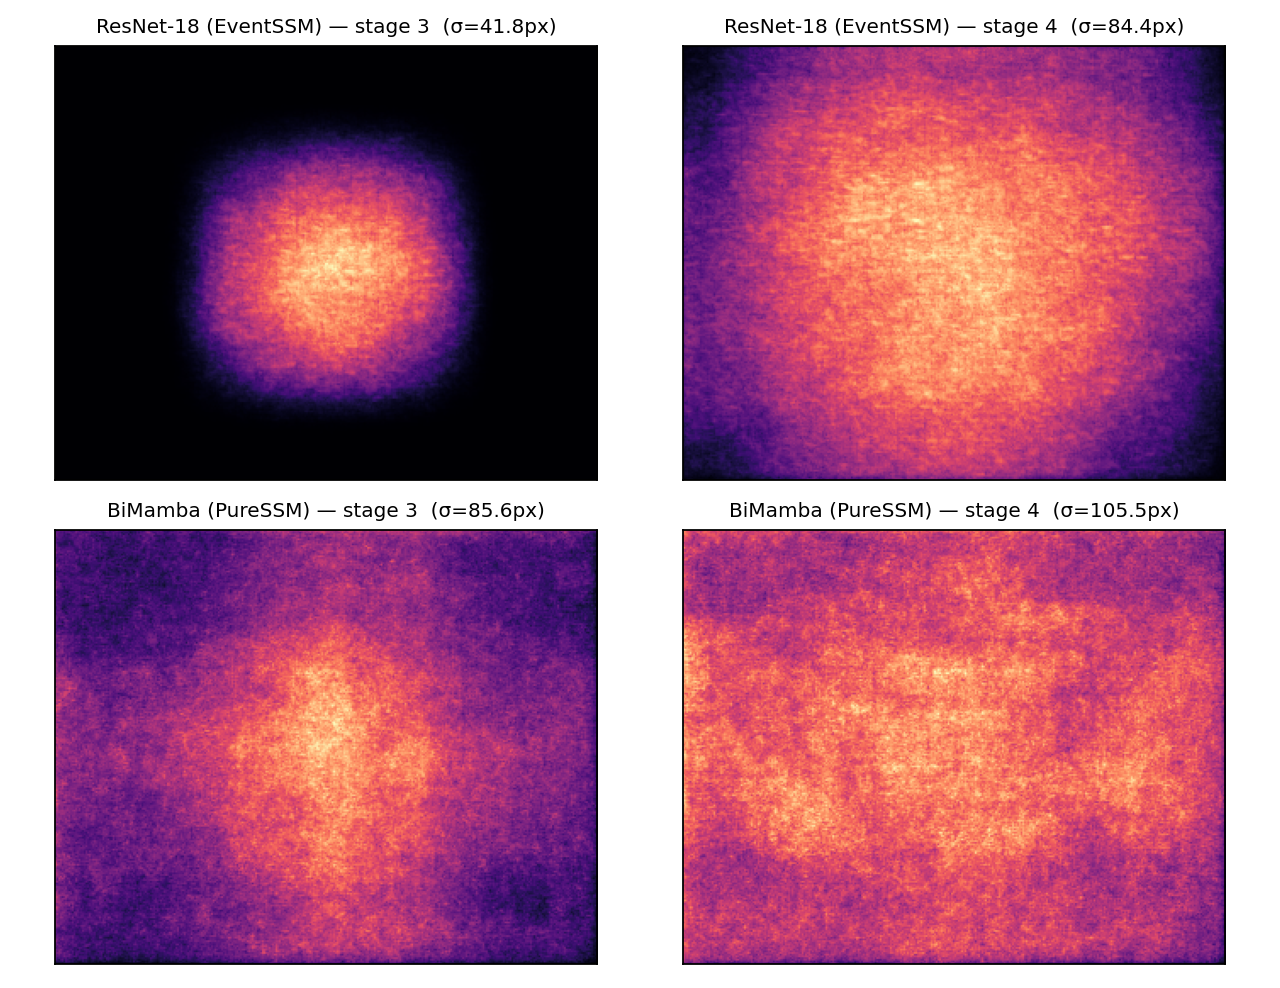
\includegraphics[width=0.85\textwidth]{images/fig_erf_trained.png}
    \caption{Effective receptive field of the trained spatial backbones at the frame centre, stages 3
    and 4: gradient magnitude of the centre feature with respect to the input (log colour scale, averaged
    over 8 random inputs). $\sigma$ is the RMS spatial spread in input pixels. The BiMamba field is wider
    at both stages and less concentrated on the centre.}
    \label{fig:erf}
\end{figure}

The difference has a structural explanation. In a convolutional stack the effective receptive field is
governed by kernel size and depth: it is approximately Gaussian and its extent grows only with the
square root of the number of layers~\cite{luo2016understanding}, so training reshapes it little, here
by 0.2~px at stage~3 and 6.2~px at stage~4. In a scan, every token can influence every other token
through the forward and backward passes, and how far that influence reaches is set by the learned decay
rates and step sizes of Equation~\eqref{eq:mamba2_state}. Training can lengthen it, and here widened it
by 30--34~px. The state-space mixer's spatial reach is therefore a learned quantity, whereas the
convolutional one is largely fixed by the architecture. Notably, the untrained BiMamba field is no wider
than the ResNet's at stage~4 (75.4 against 78.2~px): the advantage is acquired in training, not built
in. Two caveats apply. The probe uses random inputs rather than event data, and the untrained reference
for ResNet-18 is a random initialisation rather than the ImageNet weights from which EventSSM was
fine-tuned, so its $\Delta$ spans both pre-training and Gen1 training.

\section{Temporal Robustness}
\label{sec:robustness}

\subsection{Regime 1 --- fixed cadence, variable accumulation window}
\begin{table}[htbp]
\centering
\caption{Accumulation-window sweep (COCO mAP $\times$ 100). Training operating point is $1\times$.
PureSSM is given to two decimals; its $1\times$ value (46.45) is measured on the re-preprocessed test set
used for the sweep and differs from the canonical 46.43 only through that preprocessing.}
\label{tab:regime1}
\begin{tabular}{llccc}
\toprule
\textbf{Multiplier} & \textbf{$\Delta t$} & \textbf{S5-RVT} & \textbf{EventSSM} & \textbf{PureSSM} \\
\midrule
$0.25\times$ & 200\,ms & 41.0 & 40.9 & \textbf{41.65} \\
$0.5\times$  & 100\,ms & 46.5 & 45.5 & 45.67 \\
$1\times$    & 50\,ms  & 47.7 & 46.2 & 46.45 \\
$2\times$    & 25\,ms  & 45.0 & 43.5 & 44.09 \\
$4\times$    & 12.5\,ms & 38.4 & 35.4 & 35.68 \\
\bottomrule
\end{tabular}
\end{table}

PureSSM and EventSSM are tied across this sweep, both marginally below the baseline. One result at the
dense end needs care. At the $0.25\times$ window PureSSM exceeds the baseline overall ($+0.7$, 41.65 against 40.95), driven
by large objects: on the smeared dense frames the attention baseline's $\mathrm{AP}_L$ falls by 14.3 and
PureSSM's by 7.7, leaving PureSSM 3.58 ahead on $\mathrm{AP}_L$. The overall margin is too small to
distinguish with single runs; the $\mathrm{AP}_L$ difference is the larger effect. PureSSM is therefore more robust at the dense,
slow end of the sweep and the baseline at the sparse, fast end.

\subsection{Regime 2 --- true rate change}
\begin{table}[htbp]
\centering
\caption{True event-rate change. Retention $=\mathrm{mAP}@\text{rate} \div \mathrm{mAP}@1\times$.
$^{\dagger}$Published by Zubic et al.~\cite{zubic2024state} for RVT at 200\,Hz, obtained with
preprocessing that was not released; not measured on this test set (Section~\ref{subsec:f2}).}
\label{tab:regime2}
\begin{tabular}{lcccc}
\toprule
 & \textbf{S5-RVT} & \textbf{EventSSM} & \textbf{ConvLSTM}$^{\dagger}$ & \textbf{PureSSM} \\
\midrule
true-$10\times$ mAP        & 29.67 & 29.09 & 8.35 & \textbf{32.38} \\
true-$10\times$ retention  & 62.2\% & 63.0\% & 17.7\% & \textbf{69.7\%} \\
true-$2\times$ retention   & 95.1\% & 95.5\% & --- & \textbf{95.9\%} \\
\bottomrule
\end{tabular}
\end{table}

PureSSM is the most rate-robust model tested. Because EventSSM and PureSSM share an \emph{identical}
temporal path, the additional robustness originates in the spatial backbone. The wider receptive field
behind the $\mathrm{AP}_L$ result is a plausible explanation, since true-$10\times$ frames are event-sparse,
but it has not been tested directly.\needsgpu{decision D1: add RVT's ConvLSTM measured on this true-rate
test set, replacing the published column}

\subsection{Reproducing inference-time \texorpdfstring{$\Delta t$}{Delta t}-rescaling}
\label{subsec:f2}
Zubic et al.~\cite{zubic2024state} report that state-space detectors generalise to event rates not seen
in training when the discretisation step is rescaled at inference to match the new rate, and give
39.84~mAP on Gen1 at 200\,Hz (a tenfold rate increase) for S5 with this compensation, against 8.35 for
RVT's ConvLSTM. This work attempted to reproduce that result with the published checkpoint and code, and
transferred the compensation to Mamba by rescaling the post-softplus step $\Delta_t$ of
Equation~\eqref{eq:mamba2_state} by the same factor. Table~\ref{tab:dt_comp} lists every compensated
evaluation in the true-rate regime.

\begin{table}[htbp]
\centering
\caption{Inference-time $\Delta t$ compensation under a true rate change (regime~2), mAP on the Gen1
test split. ``Comp.'' rescales the step by the window ratio, the convention of~\cite{zubic2024state}.
The published reference is S5 with compensation at 200\,Hz.}
\label{tab:dt_comp}
\begin{tabular}{llcccc}
\toprule
True rate & & \textbf{S5-RVT} & \textbf{EventSSM} & \textbf{PureSSM} & Published \\
\midrule
$2\times$ (25\,ms)  & no comp.  & 45.37 & 44.13 & 44.53 & --- \\
                    & comp.     & 44.51 & 43.67 & 44.13 & --- \\
\midrule
$10\times$ (5\,ms)  & no comp.  & \textbf{29.67} & \textbf{29.09} & \textbf{32.38} & --- \\
                    & comp.     & 19.96 & 20.18 & 19.70 & 39.84 \\
                    & difference & $-9.71$ & $-8.91$ & $-12.68$ & \\
\bottomrule
\end{tabular}
\end{table}

Three observations follow, all under the published artefacts. First, the compensation did not recover
accuracy at any tested operating point. In regime~1 there is nothing for it to compensate: the model's
step cadence is unchanged and only the number of events per frame falls, so rescaling $\Delta t$ only
detunes the recurrence, and accuracy peaks at the trained step. In regime~2 the compensated models score
below the uncompensated ones at both rates, by 9--13~mAP at the tenfold rate, consistently across S5 and
both Mamba models. Second, the published 200\,Hz figure could not be reproduced: the best S5 result at a
true tenfold rate is 29.67~mAP, without compensation. The released preprocessing also cannot generate a
true-rate test set, because the frame stride is fixed at 50~ms in the code; the published experiment
must therefore have used preprocessing that was not released, and that difference may account for the
discrepancy. Third, the rate robustness itself is reproduced: without any compensation every state-space
model retains 62--70\,\% of its accuracy at a true tenfold rate (Table~\ref{tab:regime2}), against the
17.7\,\% reported for the ConvLSTM under the authors' unreleased preprocessing.

The conclusion drawn here is accordingly limited to what the published artefacts support. State-space
detectors are substantially more rate-robust than the recurrent-convolutional baseline, and under the
released checkpoint and code this robustness does not require the inference-time compensation. Whether
the compensation behaves differently under the unreleased preprocessing cannot be determined from the
published material. The complete audit, with the code evidence and all evaluations, is recorded in the
project repository (\path{docs/notes/Stage9_Zubic_methodology_verdict.md}).

\section{Efficiency}
\label{sec:efficiency}
\begin{table}[htbp]
\centering
\caption{Full-pipeline streaming inference, RTX 5070 Ti, idle-GPU-guarded harness. FLOPs per frame
are counted as defined in Section~\ref{sec:eval_protocol}; mAP per GFLOP uses the test AP of
Table~\ref{tab:accuracy}.}
\label{tab:efficiency}
\begin{tabular}{lccc}
\toprule
\textbf{Metric} & \textbf{S5-RVT} & \textbf{EventSSM} & \textbf{PureSSM} \\
\midrule
Total parameters       & 18.19\,M & 19.18\,M & \textbf{16.33\,M} \\
FLOPs                  & 11.06\,G & 12.71\,G & \textbf{10.03\,G} \\
mAP per GFLOP          & 4.32 & 3.64 & \textbf{4.63} \\
Latency p50, eager     & 17.14\,ms & \textbf{12.60\,ms} & 26.86\,ms \\
Throughput, eager      & 58\,Hz & \textbf{79\,Hz} & 37\,Hz \\
Throughput, CUDA-graph & --- & \textbf{210\,Hz} & 181\,Hz \\
Energy per frame       & 0.723\,J & \textbf{0.438\,J} & 0.652\,J \\
Streaming state        & \textbf{4.7\,MB} & 144\,MB & 144\,MB \\
\bottomrule
\end{tabular}
\end{table}

The efficiency story is a trade-space, and reporting it honestly strengthens rather than weakens the
thesis. PureSSM performs the least computation with the best accuracy-per-FLOP, yet is the slowest in
eager wall-clock: its backbone is many small scan operations and is launch-overhead-bound, and
state-space scans utilise the GPU less well than cuDNN convolutions. CUDA-graph replay repairs most of
this ($37 \rightarrow 181$\,Hz, the largest speed-up of any model precisely because it was the most
launch-bound), but the fair same-mode comparison still leaves EventSSM ahead in both modes. Two further
caveats must be stated: event sparsity does \emph{not} translate into GPU speed, so the efficiency claim
is FLOP-efficiency and rate-robust deployability, not ``sparse means fast''; and the Mamba state
expansion makes the streaming state 31 times larger than the baseline's, which for a SWaP-constrained
platform is the number to watch.

\section{Qualitative Results}
\label{sec:qualitative}
To see the large-object behaviour behind the $\mathrm{AP}_L$ result, the twelve test recordings with the
most large-car instances were selected (a large car being a ground-truth car box covering at least 10\,\%
of the $304\times240$ frame), and ground-truth-versus-prediction overlay videos were rendered for both
own models. Figure~\ref{fig:qualitative} shows the top-ranked recording (180 large-car instances) as
eight evenly spaced frames, not selected by hand. The videos and the remaining eleven recordings are
reproducible from the repository (\path{code/event_ssm/scripts/stage16_render_gt_vs_pred.sh}).

\begin{figure}[htbp]
    \centering
    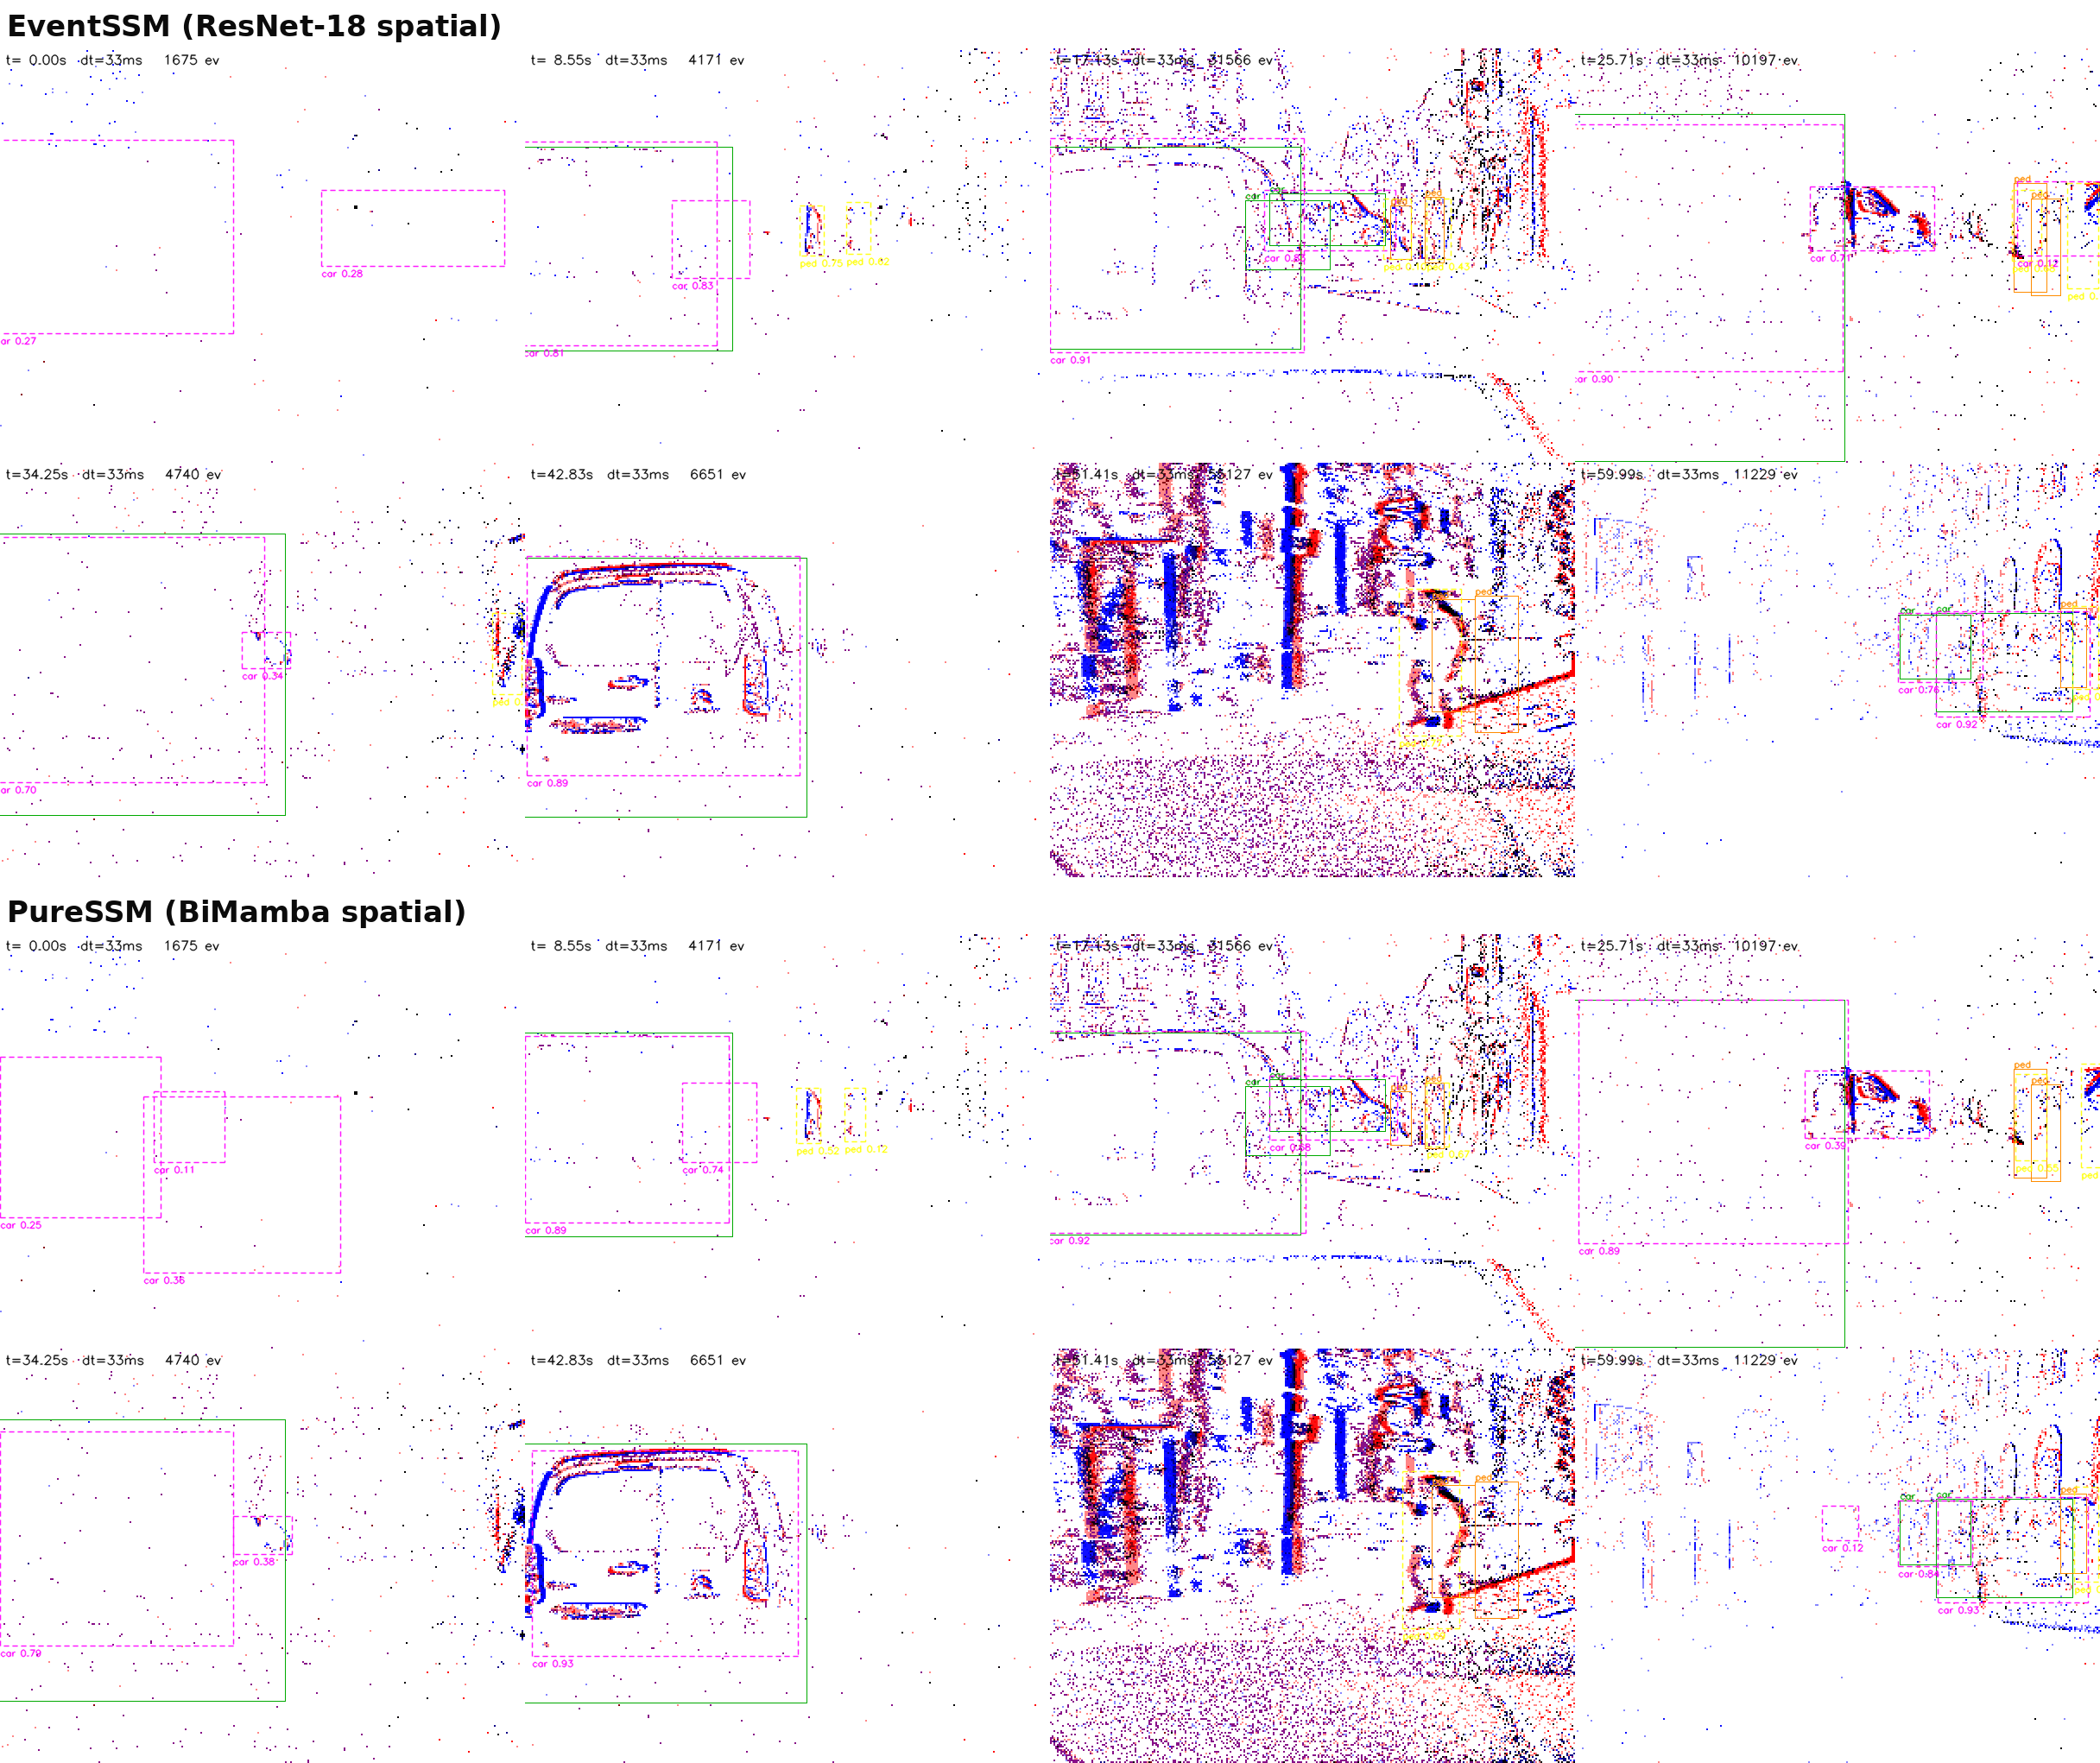
\includegraphics[width=\textwidth]{images/fig_qualitative_large_car.png}
    \caption{Ground truth against predictions on the test recording with the most large-car instances
    (\texttt{18-03-29\_13-15-02\_500000\_60500000}), eight evenly spaced frames from its 60~s; top
    EventSSM, bottom PureSSM. Events of 33~ms are drawn by polarity (red/blue). Solid boxes are ground
    truth (car green, pedestrian orange), each held for up to 250~ms after its annotation; dashed boxes
    are predictions with their confidence (car magenta, pedestrian yellow), shown down to RVT's
    default inference threshold of 0.1 (the AP evaluation itself uses 0.001).}
    \label{fig:qualitative}
\end{figure}

Four observations recur across the recordings. First, close cars that generate events are detected
by both models with high confidence (0.81--0.93 in Figure~\ref{fig:qualitative}). Second, detections
persist when the scene goes quiet. At 25.7~s and 34.3~s almost no events fall on the car, because an
event camera reports only change, yet both models keep it at 0.70--0.90 confidence: the object is
carried by the recurrent state rather than seen in the current frame. Third, at the start of a
recording, with the state still empty and few events (1{,}675 in the first frame), both models emit
low-confidence car boxes (0.1--0.4) where there is no ground truth. Fourth, the ground truth itself
flickers: with annotations about once per second (Section~\ref{sec:dataset}), a box appears in a
rendered frame only when an annotation falls within the 250~ms hold. Pedestrians and distant objects
visible in the events are frequently unlabelled; a correct detection of one counts as a false positive
and lowers the measured AP of every model. On these frames the two models behave very similarly,
as expected from their identical temporal path; the frames illustrate the behaviour, while the
difference between the models rests on the quantitative $\mathrm{AP}_L$ result of
Section~\ref{sec:acc_results}.

\section{Spiking SSM Detector}
\label{sec:spiking_results}
\needsgpu{Stages 20--22. This section is scaffolded so the writing can proceed around it.}

\tbd{Report, in this order: (i) Gen1 test mAP, positioned against the published SNN detectors as
\emph{context} --- but state explicitly that this model is a \textbf{hybrid} (spiking temporal readout,
non-spiking spatial backbone) and therefore not a like-for-like competitor to the full-spike architectures
in Table~\ref{tab:snn_landscape}. Do NOT frame the result as beating or failing to beat SNN SOTA; that axis
is wrong in both directions. (ii) the three-readout
decomposition (spike / graded / analog), which separates the cost of sparsity from the cost of
binarisation --- note that the analog arm shares the spiking membrane (leak and subtract-reset), so the
step from PureSSM to the analog arm measures the cost of the neuron dynamics themselves, while integration
correctness is established separately by the null test (\texttt{spiking\_stages = []} is numerically identical
to PureSSM); (iii) firing rate and spike sparsity per stage; (iv) SOPs and the estimated energy,
with the ANN-MAC versus SNN-SOP model stated explicitly, since sloppy energy accounting is the standard
reviewer target.}

\begin{table}[htbp]
\centering
\caption{Spiking readout ablation on Gen1 (to be completed).}
\label{tab:spiking_ablation}
\begin{tabular}{lcccc}
\toprule
\textbf{Readout} & \textbf{mAP} & \textbf{Firing rate} & \textbf{SOPs} & \textbf{Energy / frame} \\
\midrule
analog (dense LIF) & --- & n/a & n/a & --- \\
graded           & --- & --- & --- & --- \\
spike (binary)   & --- & --- & --- & --- \\
\bottomrule
\end{tabular}
\end{table}


\chapter{Discussion}
\label{ch:discussion}

\section{What the Four Models Show}
\label{sec:what_shown}
\textbf{A pure state-space spatial backbone is a viable detection backbone.} PureSSM uses no attention,
and apart from strided downsampling convolutions its only local spatial mixing is a zero-initialised
depthwise term in each block. It nonetheless
matches the convolutional hybrid on overall accuracy (46.43 against 46.22, Table~\ref{tab:accuracy})
with the fewest parameters (16.33\,M) and the fewest FLOPs (10.03\,G) of the three models, and it is the
most robust of them to a true change in event rate (69.7\,\% retention at a tenfold rate,
Table~\ref{tab:regime2}). Two qualifications keep this in proportion. It remains 1.3~mAP below the
attention-based baseline, and its rate advantage holds for a true rate change: under a fixed cadence
with a shortened accumulation window, the baseline degrades least (Table~\ref{tab:regime1}).

\textbf{The receptive field is the lever.} One controlled change, the spatial mixer, raises large-object
accuracy by 2.95~$\mathrm{AP}_L$ while small- and medium-object accuracy barely moves ($+0.08$ and
$+0.28$). The receptive-field probe explains the pattern: the state-space mixer learns a field twice as
wide as the convolutional stack's at stage~3 and a quarter wider at stage~4, while the convolutional
field changes little in training (Section~\ref{sec:erf}). The class-level result agrees, since the gain
is in cars, the class with large and close instances, and not in pedestrians. The same wider field is
the most plausible source of PureSSM's additional rate robustness, because EventSSM and PureSSM share an
identical temporal path; that attribution follows from the controlled design rather than from a direct
probe.

\textbf{State-space temporal processing is robust to the event rate.} All three state-space models
keep 62--70\,\% of their accuracy at a true tenfold rate without any compensation, against 17.7\,\%
reported for the ConvLSTM under the authors' unreleased preprocessing (Table~\ref{tab:regime2}). Under the published artefacts this robustness does
not depend on the inference-time $\Delta t$ compensation, which lowered accuracy at every tested
operating point (Section~\ref{subsec:f2}); whether it behaves differently under the unreleased
preprocessing cannot be settled from the released material. For a platform whose event rate varies with
its own speed, the practical consequence is that a state-space detector degrades gracefully, rather than
collapsing, at a rate it was not trained for, and without per-rate tuning.

\textbf{Efficiency is a trade-space, not a free gain.} PureSSM performs the least computation and has
the best accuracy per FLOP, but it is the slowest model in eager execution (37\,Hz), because its
fourteen bidirectional scans launch many small kernels. CUDA-graph replay lifts it to 181\,Hz, yet
EventSSM stays ahead in both modes (79 and 210\,Hz) and draws the least energy per frame (0.438\,J). The
baseline carries a 4.7\,MB streaming state against 144\,MB for both Mamba models, the cost of Mamba's
state expansion at every spatial location. Event sparsity does not help on the GPU at all: every frame
is processed densely, whatever its event count. Which model is most efficient therefore depends on the
binding constraint (FLOPs, latency, energy or memory), and the thesis reports the frontier rather than
a winner on any single axis.

\textbf{PureSSM and EventSSM are two legitimate designs.} Published state-space event detectors keep a
conventional mixer on one of the two axes: S5-RVT combines attention in space with an S5 recurrence in
time~\cite{zubic2024state}, and SMamba a sparse spatial Mamba with a ConvLSTM in time~\cite{yang2025smamba}.
EventSSM follows the same pattern, pairing a lightweight convolutional spatial mixer with Mamba in time.
PureSSM is state-space on both axes. It buys a smaller model, fewer FLOPs, better large-object accuracy
and greater rate robustness, and pays in wall-clock latency on current GPUs. Which is preferable depends
on whether a deployment is bound by computation and robustness, or by latency on conventional hardware.

\section{The Neuromorphic Case}
\label{sec:neuro_case}
The neuromorphic strand rests on three properties that the GPU measurements of
Section~\ref{sec:efficiency} cannot capture. First, the event sparsity that a GPU leaves unused is what
neuromorphic processors are built for: they compute only when spikes arrive, so their energy scales with
activity rather than with frame size~\cite{davies2021advancing}. Second, the temporal core of the models
in this thesis is a linear recurrence with a diagonal decay (Equation~\eqref{eq:mamba2_state}), which
decomposes into independent per-state updates, each implementable as a neuron. Loihi~2 supports
user-programmable neuron models through microcode~\cite{orchard2021efficient}, and Meyer
et al.~\cite{meyer2024diagonal} mapped the diagonal SSM S4D onto it, measuring for token-by-token
processing about 1000 times less energy and 75 times lower latency than a recurrent S4D implementation on
a Jetson Orin Nano. Third, Loihi~2 supports graded spikes, which carry an integer payload rather than a
single bit~\cite{orchard2021efficient}. They are the hardware counterpart of the graded readout of
Section~\ref{subsec:readout_modes} and address the binary information bottleneck that the spike readout
imposes; Section~\ref{sec:spiking_results} measures what that bottleneck costs.

Three gaps separate the model of this thesis from silicon. (i) Mamba's step $\Delta_t$ is input
dependent, so its decay $\exp(\Delta_t a)$ changes at every step. The S4D port relies on fixed, linear
time-invariant dynamics, and a selective recurrence would need either per-step computation of the decay
on the chip or a fixed-step variant. (ii) Only the temporal readout spikes; the BiMamba spatial backbone
is not spiking (Section~\ref{subsec:spiking_method}) and would run on a conventional accelerator, so the
deployed system would be hybrid. (iii) The software path is in flux. Intel archived the Lava framework on
13 May 2026, stating that it will no longer maintain it, and has announced a successor SDK without a
public timeline~\cite{intel2026lava}. This thesis therefore uses the Neuromorphic Intermediate
Representation (NIR)~\cite{pedersen2024neuromorphic}, a vendor-neutral exchange format, as its export
boundary, so that the model can be retargeted to Lava's successor or to another neuromorphic platform.
The energy figures of Section~\ref{sec:spiking_results} are accordingly estimates from operation counts
in simulation, not measurements on hardware.

\section{Scope Change: the Obstacle-Avoidance Aim}
\label{sec:scope_change}
The fourth aim registered in Thesis~A --- integration with an obstacle-avoidance controller in
simulation, and physical micro-UAV testing if feasible --- was not undertaken. It was to be evaluated by
collision rate, avoidance latency and trajectory smoothness in AirSim or Gazebo. Two parts of the second
aim were also not delivered: the 1Mpx dataset and latency on embedded hardware. Table~\ref{tab:aims} sets
every registered aim against what this thesis delivers.

\begin{table}[htbp]
\centering
\small
\caption{Aims registered in Thesis~A against what was delivered.}
\label{tab:aims}
\begin{tabularx}{\textwidth}{@{}l>{\raggedright\arraybackslash}X>{\raggedright\arraybackslash}X@{}}
\toprule
\textbf{Aim} & \textbf{Registered} & \textbf{Delivered} \\
\midrule
1 Architecture & SSM detector, comparing S4/S5/Mamba variants &
  Delivered: two Mamba detectors (EventSSM, PureSSM) and a spiking variant, compared against the S5
  baseline (Chapter~\ref{ch:method}). \\
2 Benchmarking & Gen1 and 1Mpx; accuracy, latency, memory, energy; CNN, RNN and transformer baselines;
  embedded-hardware latency &
  Delivered on Gen1 with all four metrics (Sections~\ref{sec:acc_results}, \ref{sec:efficiency}); the
  RNN (ConvLSTM) baseline enters only through its published rate result.\needsgpu{decision D1: replace with
  the measured ConvLSTM baseline}
  1Mpx deferred to future work (Section~\ref{sec:future_work}); latency and energy measured on a
  desktop GPU, not embedded hardware. \\
3 Temporal generalisation & Inference at frequencies other than training, without retraining &
  Delivered and extended to two regimes, fixed cadence and true rate change, including a reproduction
  of inference-time $\Delta t$-rescaling (Section~\ref{sec:robustness}). \\
4 System integration & Obstacle-avoidance controller in simulation; micro-UAV flight if feasible &
  Descoped (this section). \\
\bottomrule
\end{tabularx}
\end{table}

The descope follows from what a closed-loop demonstration could and could not have measured. The
detector is trained and evaluated on Gen1, recorded by a car-mounted $304\times240$ sensor with car and
pedestrian classes. An avoidance loop needs obstacles detected from a UAV's viewpoint. Integrated in a
simulator, the Gen1 detector would have faced objects and viewpoints it was never trained on, and the
labelled UAV-related event datasets identified in this project's survey address the inverse problem of
detecting drones from the ground rather than obstacles from the drone. A collision rate obtained under
those conditions would have measured the domain gap, the controller and the simulator together, and
could not have isolated the contribution of the state-space backbone, which is the question this thesis
sets out to answer (Section~\ref{sec:rq}). The aim also depended on assets outside the project's
control: event-camera simulation plugins, a stereo event sensor whose integration remained unresolved,
micro-UAV hardware and flight approvals. Each additional model, by contrast, required about 30
GPU-hours of training on a fixed pipeline under the project's own control.

The effort was therefore redirected into the controlled architectural study. It produced a mechanism
for the large-object result, in which the state-space spatial mixer learns a receptive field up to twice
as wide as the convolutional stack's (Section~\ref{sec:erf}); a two-regime study of rate robustness that
reproduces the robustness itself but not the inference-time compensation credited with it
(Section~\ref{sec:robustness}); and an efficiency frontier that includes the results unfavourable to the
proposed models (Section~\ref{sec:efficiency}). None of these would have come out of a simulated avoidance
demonstration, whose outcome depends on many components other than the backbone.

The micro-UAV motivation is unchanged; what changed is that the evaluation is architectural rather than
system-level. Several results bear on that motivation directly. The event rate of a moving camera varies
with its speed and the scene~\cite{gallego2020event}, so robustness to rate changes is a property a
flying platform needs, and PureSSM is the most rate-robust model tested. Parameters, FLOPs, latency and
energy are reported for every model, including the 31-fold larger streaming state of the Mamba models,
which counts against them on a memory-constrained platform. The spiking model opens a path to
neuromorphic hardware, whose energy is estimated here in simulation rather than measured on silicon
(Section~\ref{sec:spiking_results}). What the thesis does not show is how any of the detectors behaves in
a closed loop; that remains future work (Section~\ref{subsec:fw_closed_loop}).

\section{Limitations}
\label{sec:limitations}
\begin{itemize}
  \item \textbf{Single seed, no error bars.} Each model was trained once, so run-to-run variation is
        unmeasured. Overall-mAP differences below about 1~mAP are treated as not distinguishable; larger
        effects, such as the $\mathrm{AP}_L$ gain and the robustness gaps, are reported, but they also rest
        on single runs. A second seed of the own models would bound the variation.
  \item \textbf{One dataset.} All results are on Gen1: low resolution, an automotive viewpoint, two classes, ego-motion.
        Generalisation across resolution, domain and conditions is untested.
  \item \textbf{Label noise} in Gen1 caps achievable AP and adds a qualitative confound.
  \item \textbf{Fixed representation.} Every model inherits the stacked-histogram tokeniser; the
        representation is not part of the ablation.
  \item \textbf{Precision mix} --- bf16 mixed precision for the own models against 32-bit training for
        the published baseline (Table~\ref{tab:recipe}). Its effect on accuracy was not measured; like the
        batch size, it affects only the comparison against the baseline.
  \item \textbf{Initialisation of the spatial mixers.} EventSSM's ResNet-18 starts from ImageNet weights,
        while PureSSM's BiMamba stack is trained from scratch with stochastic depth. The EventSSM--PureSSM
        comparison therefore isolates the spatial mixer \emph{as instantiated}, including its
        initialisation. Pre-training would be expected to favour the convolutional model, so it is unlikely
        to explain PureSSM's large-object gain, but the two factors are not separated.
  \item \textbf{Half the baseline's batch size.} The own models trained at batch 4 against the published
        baseline's 8 (Section~\ref{sec:training}), so they saw half as many training sequences. The
        own-model-to-baseline gap may therefore be overstated; comparisons among own models are
        unaffected.
  \item \tbd{spiking-specific limitations once Stage 20--22 have run --- binary information bottleneck,
        surrogate-gradient sensitivity, and the fact that energy is estimated rather than measured on
        silicon.}
\end{itemize}


\chapter{Conclusion and Future Work}
\label{ch:conclusion}

\section{Summary of Contributions}
This thesis asked what the spatial mixer of an event-camera detector's backbone contributes when
everything else is held fixed. The contributions listed in Section~\ref{sec:contributions} were achieved
as follows.

\begin{enumerate}
  \item \textbf{A verified baseline.} The published S5-RVT checkpoint reproduces at Gen1 test mAP 47.72
        ($\mathrm{AP}_{50}$ 75.28), an exact match, which validates the pipeline, preprocessing and
        evaluator used for every other number in this thesis (Section~\ref{sec:baseline_repro}).
  \item \textbf{Two original detectors in a controlled ablation.} EventSSM (ResNet-18 spatial, Mamba-2
        temporal) reaches 46.22~mAP and PureSSM (bidirectional Mamba spatial, identical temporal path)
        46.43, trained with one recipe through the same unmodified pipeline, so that their difference is
        attributable to the spatial mixer as instantiated, including its initialisation
        (Section~\ref{sec:acc_results}).
  \item \textbf{A mechanism for the large-object result.} Replacing the convolutional spatial mixer with
        a state-space one raises $\mathrm{AP}_L$ from 44.70 to 47.65, closing about half of EventSSM's
        large-object gap to the baseline. The state-space mixer's effective receptive field is twice as
        wide at stage~3 (85.6 against 41.8~px) and grew by 30--34~px in training, against at most 6.2~px
        for the convolutional stack (Section~\ref{sec:erf}).
  \item \textbf{A reproduction study of $\Delta t$-rescaling.} Without compensation, the state-space
        models retain 62--70\,\% of their accuracy at a true tenfold event-rate increase, PureSSM the most
        (69.7\,\%), against 17.7\,\% reported for a ConvLSTM under the authors' unreleased preprocessing. Under
        the published checkpoint and code, the
        inference-time compensation did not recover accuracy at any tested point and cost 9--13~mAP at the
        tenfold rate, and the published 200\,Hz result (39.84) could not be reproduced; the best
        reproduction was 29.67 (Section~\ref{sec:robustness}).
  \item \textbf{An efficiency frontier.} PureSSM is the smallest model (16.33\,M parameters) with the
        fewest FLOPs (10.03\,G) and the best accuracy per GFLOP (4.63), but the slowest in eager execution
        (37\,Hz, 181\,Hz with CUDA-graph replay); EventSSM is the fastest (79 and 210\,Hz) and uses the least
        energy per frame (0.438\,J); both Mamba models carry a 144\,MB streaming state against the
        baseline's 4.7\,MB (Section~\ref{sec:efficiency}).
  \item \textbf{A spiking state-space detector.} A spiking variant whose temporal readout is a
        leaky integrate-and-fire layer, with three readout modes that decompose the cost of spiking, was
        built as a drop-in backbone for the same pipeline and verified by tests, including that it reduces
        numerically to PureSSM when no stage spikes (Section~\ref{subsec:spiking_method}).
        \needsgpu{state its headline numbers here (mAP per readout, firing rate, SOPs, estimated energy)
        once Stages 21--22 have run.}
\end{enumerate}

Taken together, the results show that a state-space model can serve as the spatial mixer as well as the
temporal one, that its advantage lies where its learned receptive field predicts, and that its efficiency
must be judged against the constraint that binds a given deployment rather than on a single axis.

\section{Future Work}
\label{sec:future_work}

\subsection{High-resolution generalisation}
Every result here is on Gen1 at $304\times240$. The natural next dataset is the Prophesee 1Mpx
dataset~\cite{perot2020learning}, recorded at $1280\times720$ (about 12.6 times Gen1's pixel count) with
car, pedestrian and two-wheeler labels. It would test whether the large-object and receptive-field
advantage of the state-space spatial mixer grows with resolution, where objects span more pixels and the
spatial scans become longer. The question should be posed as a falsifiable hypothesis rather than an
expectation that more pixels help. Gehrig and Scaramuzza~\cite{gehrig2022high} show that at high speed and
in low light, higher-resolution event cameras produce more temporal noise, because each pixel fires more
often, and can be outperformed by lower-resolution ones; learning-based methods trained on realistic,
noisy data largely overcome that penalty. The state-space detectors of this thesis retained 62--70\,\% of
their accuracy at a tenfold rate change (Section~\ref{sec:robustness}), so the hypothesis is that they
lose least to the temporal noise of a high-resolution sensor and therefore gain most from its resolution.
The models should be trained on 1Mpx rather than transferred from Gen1 without retraining; zero-shot
transfer would confound the change of resolution with the temporal-noise penalty that training on the
target data removes.

\subsection{Closed-loop evaluation on a UAV}
\label{subsec:fw_closed_loop}
The descoped fourth aim (Section~\ref{sec:scope_change}) becomes meaningful once a detector is trained on
data from a UAV's viewpoint. The order of work would be: a labelled onboard event dataset or a simulator
with event-camera rendering and obstacle labels; a detector from this thesis retrained on it through the
same frozen pipeline; and only then an avoidance controller, evaluated by collision rate and avoidance
latency. The rate-robustness result of Section~\ref{sec:robustness} predicts which backbone should degrade
least as flight speed, and hence event rate, varies; a closed-loop study could test that prediction
directly.

\subsection{Neuromorphic deployment}
The spiking detector is evaluated in simulation in this thesis; running it on Loihi~2 is the natural
continuation. Access to Intel's neuromorphic hardware is through the Intel Neuromorphic Research
Community (INRC). Research memberships are held by a principal investigator who is a permanent employee of
a research organisation; students are added to an existing project, and the participation agreement is
executed between Intel and the organisation rather than the individual~\cite{intel2026inrc}. The concrete
path is therefore: the supervisor applies as principal investigator with a project proposal, for which a
two-page draft has been prepared; the model is exported through NIR~\cite{pedersen2024neuromorphic}; it is
benchmarked first through the remote access to Intel's neuromorphic research cloud that membership
provides, and dedicated hardware is requested only afterwards. Two technical steps from
Section~\ref{sec:neuro_case} lie on this path: a fixed-step or on-chip-computed form of the selective
decay, and a decision on where the non-spiking spatial backbone runs. The toolchain itself is a live
risk. With Lava archived and its successor SDK unscheduled~\cite{intel2026lava}, the NIR export boundary
is what keeps the work retargetable.

\subsection{Representation and tokenisation}
Every model in this thesis inherits the same fixed tokeniser, a 20-channel stacked histogram over 50-ms
windows, so the representation lies outside the ablation (Section~\ref{sec:limitations}). Two directions
follow. Learned representations, such as the event spike tensor~\cite{gehrig2019end}, could replace the
fixed histogram within the same frozen pipeline. More promising is activity-driven tokenisation, which
processes only the regions where events occur, as in the token selection of SMamba~\cite{yang2025smamba}
or in asynchronous sparse and graph-based detectors~\cite{messikommer2020event,schaefer2022aegnn}.
Section~\ref{sec:what_shown} found that event sparsity brings no speed-up on a GPU, because every frame is
processed densely; a tokeniser that skips inactive regions would turn that sparsity into saved
computation. A state-space backbone suits a variable number of tokens per frame, since a scan accepts
sequences of any length, and its rate robustness matters here as well, because the number of active
tokens rises and falls with the event rate.

\subsection{Toward a fully spiking detector}
\label{subsec:fw_fullspike}
The detector reported here is a \textbf{hybrid}: the temporal readout spikes, the spatial mixer does not.
This is a deliberate design choice rather than a limitation of effort --- the governing principle is to
\emph{spike the axis that is actually time}. Spikes are causal events in time, and the temporal block
already unrolls over clip time, so the readout adds no timestep dimension; fully spiking detectors must
introduce an artificial one and pay a multiplicative compute cost for it (SpikeYOLO uses four or five timesteps, Table~\ref{tab:snn_landscape}).

Extending to a fully spiking model therefore runs into a specific, nameable obstacle rather than a merely
practical one: the spatial mixer is a \emph{bidirectional} scan whose sequence axis is space, not time.
A spiking neuron is defined by causal integration along a temporal axis, so ``spiking'' a non-causal spatial
scan is not well defined without either (i) making the spatial scan unidirectional and treating its
traversal order as pseudo-time --- which discards the global context that produced this thesis's
large-object result --- or (ii) adopting a neuron whose state dynamics \emph{are} the structured recurrence,
so that space and time are handled by one mechanism.

Option~(ii) has a concrete starting point. SiLIF~\cite{fabre2025silif} makes the correspondence between a
leaky integrate-and-fire neuron and a diagonal state-space model exact for a two-state adaptive neuron, and
gives that neuron an S4-style parametrisation: continuous-time decays trained in logarithmic form, a
learnable per-neuron discretisation step and, in a complex-valued variant, oscillatory dynamics. It reports
state-of-the-art accuracy among spiking neuron models on speech benchmarks. A SiLIF-type neuron whose state
\emph{is} the structured recurrence could replace both the temporal Mamba block and its LIF readout, so that
time is handled by a single spiking mechanism. The open problem is the spatial axis: SiLIF neurons
integrate causally, as every spiking neuron does, so a bidirectional spatial scan would still have to be
expressed as two causal passes over a traversal order treated as pseudo-time, and whether that preserves
the global context behind the large-object result is untested.

Two experiments would most sharpen the present contribution. The first is whether spiking preserves the
rate robustness of Section~\ref{sec:robustness}. The spiking readout integrates over the same clip time as
the Mamba block, but its leak and threshold are learned at the training rate, and it is not known whether
they transfer to a tenfold rate change as well as the uncompensated recurrence does. The second is where in
the backbone hierarchy spiking costs most. The implementation already allows spiking to be enabled stage by
stage, from stage~4 alone to stages 3--4 and stages 2--4, so the cost per stage can be measured directly
with the same recipe.

\chapter*{Acknowledgments}
\addcontentsline{toc}{chapter}{Acknowledgments}
The author gratefully acknowledges the guidance and support of Will Midgley in shaping the direction of
this research. Thanks are also extended to the staff of the School of Mechanical and Manufacturing
Engineering at UNSW Sydney for providing access to computational resources and laboratory facilities.

\appendix

\chapter{Mathematical Formulations}
\label{app:maths}

\section{Continuous-Time SSM}
A classical linear SSM evolves a latent state vector $h(t) \in \mathbb{R}^N$ according to a continuous-time linear dynamical system \cite{gu2022efficiently, gu2023mamba}:
\begin{align}
    h'(t) &= A h(t) + B u(t) \\
    y(t) &= C h(t) + D u(t)
\end{align}
where $u(t) \in \mathbb{R}$ is the scalar input, $y(t) \in \mathbb{R}$ is the scalar output, and $h(t) \in \mathbb{R}^N$ is the latent state. $A \in \mathbb{R}^{N \times N}$ is the state transition matrix, typically initialised via the HiPPO framework \cite{gu2022efficiently} to capture long-range history, while $B, C,$ and $D$ are learned projection matrices. The dimension $N$ controls the memory capacity of each SSM layer.

\section{Discretisation}
The continuous system is discretised at step size $\Delta$ using the zero-order hold (ZOH) method \cite{gu2023mamba}:
\begin{align}
    \overline{A} &= \exp(\Delta A) \\
    \overline{B} &= (\exp(\Delta A) - I) A^{-1} B
\end{align}
The resulting discrete recurrence is:
\begin{align}
    h_k &= \overline{A} h_{k-1} + \overline{B} u_k \\
    y_k &= C h_k + D u_k
\end{align}
This recurrence has time complexity $O(L \times N \times D)$ per layer for sequence length $L$, compared to the quadratic complexity $O(L^2 D)$ of self-attention.

\section{Mamba Selective Scan}
The selective SSM (Mamba \cite{gu2023mamba}) introduces input-dependency to the parameters $\Delta, B,$ and $C$:
\begin{equation}
    \Delta_k, B_k, C_k = f_\theta(u_k)
\end{equation}
where $f_\theta$ denotes learned linear projections. Input-dependent $\Delta_k$ enables selective retention: a large $\Delta_k$ causes rapid state decay (forgetting irrelevant content), while a small $\Delta_k$ preserves long-range memory.

\section{Event Representations}
\subsection{Stacked Histogram (used by every model)}
\label{subsec:stacked_hist}
Every model in this thesis consumes the stacked histogram of the RVT preprocessing~\cite{gehrig2023recurrent}.
For each output frame, the events $e_k=(x_k,y_k,t_k,p_k)$ with polarity $p_k\in\{0,1\}$ in the 50-ms window
ending at the frame's timestamp are assigned to one of $B=10$ temporal bins by their normalised time,
\begin{equation}
  b_k = \min\!\left(\left\lfloor B\,\frac{t_k - t_{\min}}{\max(t_{\max}-t_{\min},\,1)}\right\rfloor,\; B-1\right),
  \label{eq:sh_bin}
\end{equation}
where $t_{\min}$ and $t_{\max}$ are the first and last event timestamps in the window, in microseconds. The
events are then counted per polarity, bin and pixel, and each count is clipped at $c=10$:
\begin{equation}
  S_{p,b}(x,y) = \min\!\left(c,\; \sum_k \mathbb{1}[p_k=p]\,\mathbb{1}[b_k=b]\,\mathbb{1}[x_k=x]\,\mathbb{1}[y_k=y]\right).
  \label{eq:sh_count}
\end{equation}
The two polarities and ten bins are stacked polarity-major into $2B=20$ channels (channel $pB+b$), giving
a tensor of shape $(20,240,304)$ stored as 8-bit integers. The data pipeline converts it to floating point
without further normalisation and zero-pads it to $(20,256,320)$. Unlike the voxel grid below, events are
not interpolated between bins, and the two polarities occupy separate channels rather than being summed
with a sign. The representation is very sparse: in a sampled test recording only about 0.1\,\% of its
entries are non-zero, and the count cut-off of 10 is reached by a negligible fraction of them.

\subsection{Voxel Grid (proposed in Thesis A; not used)}
The Thesis~A plan proposed the voxel grid below. It is retained for reference only; no model in this
thesis uses it.
Event streams are converted to a $B$-bin voxel grid $V \in \mathbb{R}^{B \times H \times W}$. Each event $e_k = (x_k, y_k, t_k, p_k)$ contributes to bin $b$ via bilinear temporal interpolation \cite{zhu2019unsupervised}:
\begin{equation}
    V_b(x, y) = \sum_k p_k \cdot \max(0, 1 - |(B-1) \cdot t_k / T - b|) \cdot \delta(x-x_k) \cdot \delta(y-y_k)
\end{equation}
where $T$ is the total window duration, $B=10$ bins for the Gen1 dataset, and $\delta$ selects the matching pixel position. In the Thesis~A proposal, each bin was additionally to be normalised to zero mean and unit variance.

% --- Appendix C: Draft Thesis Outline ---

\chapter{Reproducibility}
\label{app:repro}
This appendix lists what is needed to reproduce the results of Chapter~\ref{ch:results}; the procedures
themselves are in the project repository.

\textbf{Environment.} All runs used one conda environment, pinned in \path{env/} (conda specification,
\texttt{pip} lock file, and a separate lock for the Mamba kernels). Table~\ref{tab:env} lists the
versions that matter.

\begin{table}[htbp]
\centering
\small
\caption{Pinned software environment.}
\label{tab:env}
\begin{tabular}{ll}
\toprule
Component & Version \\
\midrule
Python & 3.11.15 \\
PyTorch & 2.11.0+cu128 (CUDA 12.8, Blackwell \texttt{sm\_120}) \\
\texttt{mamba-ssm} & 2.3.2.post1, built for \texttt{sm\_120} \\
\texttt{causal-conv1d} & 1.6.2.post1, built for \texttt{sm\_120} \\
PyTorch Lightning & 2.6.5 \\
Hydra & 1.3.2 \\
\texttt{torchdata} & 0.9.0 \\
Reference implementation & \texttt{ssms\_event\_cameras} at commit \texttt{7c871b5} \\
\bottomrule
\end{tabular}
\end{table}

{\sloppy \textbf{Installation pitfalls.} The Mamba kernels must be installed with \texttt{--no-deps
--no-build-isolation}; a default installation upgrades PyTorch and its CUDA build and breaks the stack.
Loading full Lightning checkpoints under PyTorch $\geq 2.6$ requires
\path{TORCH_FORCE_NO_WEIGHTS_ONLY_LOAD=1}. The runbooks in \path{docs/runbooks/} cover a clean
local setup, the baseline reproduction, and bootstrapping a rented GPU.\par}

\textbf{Reference implementation.} The RVT/S5 code is cloned at the pinned commit and is not versioned in the
repository. Every local change to it is stored in \path{docs/patches/} and re-applied after a re-clone: the
Hydra configuration links that register the new backbones, two preprocessing fixes, and the inference-time
$\Delta t$ hook of Section~\ref{subsec:f2}.

\textbf{Tests.} The suite is run from the repository root, \texttt{pytest code/event\_ssm/tests/} (394 CPU
tests on 7 October 2026), and the GPU tests with \texttt{-m gpu} on an otherwise idle GPU (29 tests).
Running \texttt{pytest} from inside \path{code/event_ssm} instead lets the project's \texttt{models} package
shadow RVT's and produces spurious import errors.

\textbf{Checkpoints.} Table~\ref{tab:ckpts} identifies the three checkpoints behind every reported number.
Hashes were computed on 6 October 2026.

\begin{table}[htbp]
\centering
\small
\caption{Checkpoints behind the reported results (SHA-256, first 16 hex digits).}
\label{tab:ckpts}
\begin{tabular}{llll}
\toprule
Model & Origin & Selected step & SHA-256 (prefix) \\
\midrule
S5-RVT & published release~\cite{zubic2024state} & --- & \texttt{58396f15b6c6081c} \\
EventSSM & run \texttt{8zotrwjw}, workstation & 320k (best val.) & \texttt{e94a36c2157bfea0} \\
PureSSM & run \texttt{aekvsalq}, rented RTX~5090 & 310k (best val.) & \texttt{a07c108b430d288a} \\
\bottomrule
\end{tabular}
\end{table}

\chapter{Project Timeline}
\label{app:gantt}
Table~\ref{tab:timeline} and the Gantt chart below show the timeline as registered in Thesis~A. They are
retained as the plan against which the project is assessed. The ``Simulation Integration'' and ``Hardware
Testing'' phases were descoped (Section~\ref{sec:scope_change}), and the Thesis~C period was used instead
for the spiking model and the write-up.

\begin{table}[htbp]
    \centering
    \caption{Summary of the thesis timeline and major milestones, as registered in Thesis~A.}
    \label{tab:timeline}
    \renewcommand{\arraystretch}{1.4}
    \begin{tabularx}{\textwidth}{|l|X|l|}
        \hline
        \rowcolor[gray]{0.9} \textbf{Phase} & \textbf{Tasks} & \textbf{Timeline} \\ \hline
        Literature Review \& Foundations & Complete literature survey; identify optimal SSM variant and event representation. & Weeks 1--12 (Thesis A)  \\ \hline
        Architecture Design & Design SSM detection architecture; implement in PyTorch. & Weeks 13--16 (Thesis A/B)  \\ \hline
        Dataset Preparation & Download and preprocess Gen1/1Mpx datasets; implement data loaders. & Weeks 17--18 (Thesis B) \\ \hline
        Training \& Benchmarking & Train models; benchmark against baselines; ablation studies. & Weeks 18--22 (Thesis B)  \\ \hline
        Temporal Generalisation & Evaluate multi-frequency deployment; compare with RNN/Transformer. & Weeks 23--25 (Thesis B)\\ \hline
        Simulation Integration & Integrate with avoidance controller; evaluate in simulation. & Weeks 26--29 (Thesis B)\\ \hline
        Hardware Testing (if feasible) & Deploy on physical UAV platform; collect real-world results. & Weeks 30--33 (Thesis B/C)\\ \hline
        Thesis Writing & Complete thesis document; final revisions. & Weeks 34--40 (Thesis C)  \\ \hline
    \end{tabularx}
\end{table}

\begin{figure}[htbp]
    \centering
    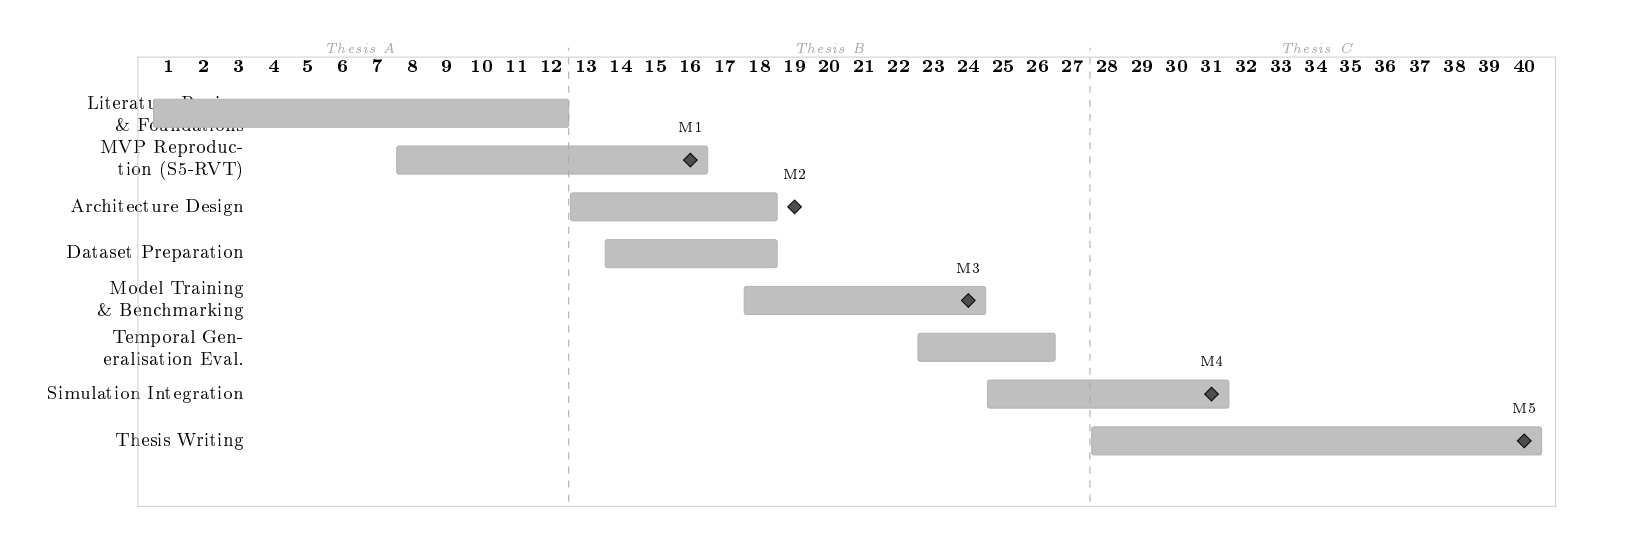
\includegraphics[width=\textwidth]{images/Ghantt Chart.png}
    \caption{Project Gantt chart showing the week-by-week schedule across all thesis phases. Thesis~A (Weeks 1--12) covers the literature review and MVP baseline reproduction. Thesis~B (Weeks 13--27) covers architecture design, dataset preparation, model training and benchmarking, temporal generalisation evaluation, and simulation integration. Thesis~C (Weeks 28--40) covers thesis writing and final submission. Diamond markers (M1--M5) indicate key milestone deliverables. The chart and Table~\ref{tab:timeline} were prepared separately in Thesis~A and differ in some week ranges; both are reproduced as registered.}
    \label{fig:gantt}
\end{figure}

% --- Appendix B: Mathematical Formulations ---

\chapter{Risk Assessment}
\label{app:risk}
Table~\ref{tab:risk_assessment} is the risk register for Thesis~C, with each risk's status on 7 October
2026. The Thesis-A risks concerning event-camera hardware, obstacle-avoidance integration and injury during
UAV flight testing were retired by the scope change of Section~\ref{sec:scope_change}, and the compute risk
by moving from the Katana cluster to a local workstation and rented GPUs of the same architecture
(Section~\ref{sec:hardware}).

\begin{table}[htbp]
    \centering
    \small
    \caption{Risk register for Thesis~C (status on 6 October 2026).}
    \label{tab:risk_assessment}
    \renewcommand{\arraystretch}{1.4}
    \begin{tabularx}{\textwidth}{|>{\RaggedRight\arraybackslash}p{3.2cm}|l|l|>{\RaggedRight\arraybackslash}X|}
        \hline
        \rowcolor[gray]{0.9} \textbf{Risk} & \textbf{Likelihood} & \textbf{Impact} & \textbf{Mitigation and status} \\ \hline
        Spiking model does not train stably & Medium & High & A kill-switch fixed before training: if the model is not training stably by 11~October, it is frozen as a simulated proof of concept and effort moves to the write-up. Spiking is introduced stage by stage, and the residual bypass is reported if used. \emph{Status:} criteria met. In overfitting tests the dense and graded readouts pass, and the binary readout, which receives about a third of the dense readout's gradient, passes with twice the steps. In 25k-step runs with spiking at stage~4 the spike and graded readouts reached 0.345 and 0.343 validation mAP against 0.351 for PureSSM under the same schedule, with no silent or saturated stage; runs with spiking at stages 2--4 are under way. \\ \hline
        Single-seed variance & High & Medium & Each model is trained once. Run-to-run variation is unmeasured; overall-mAP differences below about 1~mAP are treated as not distinguishable, and only larger effects, such as $\mathrm{AP}_L$ differences, are reported as findings, as single-seed results (Section~\ref{sec:limitations}). \\ \hline
        Training environment breaks & Medium & High & The hand-built Blackwell stack is pinned (Appendix~\ref{app:repro}); dependency resolution is disabled for the kernel packages; runbooks and patches rebuild it from scratch. \\ \hline
        Long run lost to a crash or out-of-memory kill & Medium & Medium & Full-state checkpoint resumption, validated in earlier runs; data-loader workers capped for host memory; a rented GPU of the same architecture as fallback. \\ \hline
        Write-up completed late & Medium & High & Writing runs in parallel with the experiments, and every non-spiking section is drafted before the spiking results arrive; the kill-switch caps the time the spiking strand can take. \\ \hline
        Neuromorphic hardware access delayed (INRC, Lava archived) & High & Low & Hardware deployment is future work, not a thesis result (Section~\ref{sec:future_work}); the model is exported through the vendor-neutral NIR format. \\ \hline
    \end{tabularx}
\end{table}


\addcontentsline{toc}{chapter}{References}
\bibliographystyle{ieeetr}
\bibliography{references}

\end{document}
